%%%%%%%%%%%%%%%%%%%%%%%%%%%%%%%%%%%%%%%%%%%%%%%%%%%%%%%%%%%%%%%%%%%%%%%%%%%%%%%%
\chapter{A Review: The Recovery of 3D Facial Shape From Images and Videos}\label{ch:background}
%%%%%%%%%%%%%%%%%%%%%%%%%%%%%%%%%%%%%%%%%%%%%%%%%%%%%%%%%%%%%%%%%%%%%%%%%%%%%%%%
\minitoc{}
%%%%%%%%%%%%%%%%%%%%%%%%%%%%%%%%%%%%%%%%%%%%%%%%%%%%%%%%%%%%%%%%%%%%%%%%%%%%%%%%
The recovery of 3D facial shape from images and videos has a rich history
that is closely interwoven with the more general area of generic 3D shape
recovery. Due to the many applications of 3D facial data and the
relative ease of facial data collection, many generic methods for 3D shape
recovery have given examples of reconstructions for faces. Therefore, it
becomes difficult to separate methods that focus on 3D facial shape recovery
and more generic methods that provide facial shape recovery results
amongst many other examples. This is particularly prevalent in the Structure-
from-Motion (SfM) literature whereby few papers focus solely on face recovery
yet many papers show examples of facial reconstructions. In order to provide
a thorough treatment on both the history and the current state-of-the-art for
3D facial shape recovery, it is necessary to isolate key examples
of these more generic methodologies and present their application to faces.
Furthermore, there are examples of 3D facial shape recovery across all methods
of general shape recovery given in \cref{tbl:3d_recovery_methods} and thus
the relevant literature is vast. In this section, we will attempt to provide
an exhaustive review of methods for 3D facial shape recovery and will provide
literature for both sparse and dense shape recovery, despite the focus
of this thesis being on dense recovery. Given the scope of the review, the
literature will be separated into the categories provided by
\cref{tbl:3d_recovery_methods}. Each subsection will briefly describe the
key mechanics involved for the reconstruction method but will not focus on
an exhaustive review of all of the relevant literature for a given method.
Instead, only those methods that focus on facial shape recovery or provide
representative reconstructions of faces will be considered.

The rest of this section will proceed as follows. \cref{sec:bg_db_capture} will
discuss the currently available databases of 3D facial shape in the form
of meshes and reflectance information. It will also briefly touch on recent
innovations for capturing these databases. \cref{sec:bg_sfs} provides an overview
of Shape-from-Shading (SfS) methods for facial surface normal recovery from
single images. \cref{sec:bg_ps} discusses both calibrated and
Uncalibrated Photometric Stereo methods. When discussing Uncalibrated methods,
more recent large-scale methods from Internet images are also included.
\cref{sec:bg_3dmm} presents the relevant literature for Morphable Models,
beginning with work of \citet{volker1999morphable}.
\cref{sec:bg_model_based} gives an
overview of methods that attempt to directly infer shape information from images
by using models. \cref{sec:bg_sfm} discusses Structure-from-Motion methods,
including relevant methods that provide representative reconstructions
on faces despite not leveraging facial models.
%%%%%%%%%%%%%%%%%%%%%%%%%%%%%%%%%%%%%%%%%%%%%%%%%%%%%%%%%%%%%%%%%%%%%%%%%%%%%%%%
%%%%%%%%%%%%%%%%%%%%%%%%%%%%%%%%%%%%%%%%%%%%%%%%%%%%%%%%%%%%%%%%%%%%%%%%%%%%%%%%
\section{Databases And Capture Methods}\label{sec:bg_db_capture}
%%%%%%%%%%%%%%%%%%%%%%%%%%%%%%%%%%%%%%%%%%%%%%%%%%%%%%%%%%%%%%%%%%%%%%%%%%%%%%%%
In contrast to generic shape recovery, facial shape recovery implies a strong
assumption that the input image contains a face. This prior knowledge, that the
image contains a face, enables the use of training data to improve the
quality of the reconstruction. However, collection of this training data, which
may take the form of either direct 3D information (meshes, range images) or
functions of the facial surface (normals, parametric reflectance data) must
use accurate shape recovery methods in order to be useful. Therefore, the
collection of accurate facial shape for the purposes of providing approximate
ground truth data is a research topic in its own right. In this section, we
begin by discussing the existing 3D facial databases and the manner of their
collection. Following this, we discuss the details of the 3D recovery algorithms
and focus on works intended specifically for facial surface recovery.
%%%%%%%%%%%%%%%%%%%%%%%%%%%%%%%%%%%%%%%%
% CANDIDE 3d wireframe model
% MPI     7 views, 200 laser scanned heads, 5 full 3D, Cyberware, static, neutral
% ND-D    953 scans, Minolta Vivid 900 3D scanner, 656 subjects, neutral, static
% ND-2006 13,450 images containing 6 different types of expressions, 888 distinct people
%         Static, Minolta Vivid 910 range scanner
% 3D-TEC 212 individuals (106 twins),  Minolta VIVID 910 3D scanner, 1 neutral, 1 smiling, static
% CASIA 3D 4624 scans of 123 persons, Minolta Vivid 910, various poses, emotions, static
% B3D(AC)^2 scanned using \cite{weise2007fast}, 14 subjects, 1109 sequences, dynamic 25 FPS, reading
% BIWI Head Pose  15K images of 20 people, various head poses, missing frames, kinect
% UOY Face Database 97 people, multi-pose, neutral, smile and frown
% GavabDB 61 individuals, 427 images, multi pose, static, 3 expressions
% FRAV3D 106 subjects,  MINOLTA VIVID-700, multi-pose, static
% Basel 200 scans, neutral, ABW-3D structured light scanner
% BJUT-3D, Cyberware
% EURECOM Kinect, 52 people * 18 image, multi poses, expressions, static
% XM2VTS stereo, 25 subjects, neutral,
% Texas 3DFRD 1149 pairs of facial color and range images of 105 adult human subjects,
%             stereo imaging system manufactured by 3Q Technologies, neutral, frontal
% ZJU-3DFED  40 subjects, total 360, expressions, InSpeck 3D MEGA Capturor DF
% 3D_RMA structured light, 120 people, 6 shots, multi-pose
% Beckmann cyberware, 400-500, single shot
% UMB-DB Minolta Vivid 900 laser scanner
\begin{table*}
\centering
\resizebox{\textwidth}{!}{%
\begin{tabular}{@{}lrcccccc@{}}
\toprule
\multicolumn{3}{c}{DB}                                                              & \# Subjects & \# Outputs  & Expressions & Poses & Type   \\ \midrule
CANDIDE v1                  &\cite{Rydfalk:1987tg}          & 1987                  & 1           & 1           & $\cm$       & ---   & MO     \\ \midrule
MPI                         &\cite{Troje:1996ep}            & 1996                  & 200         & 200         &             &       & M      \\ \midrule
CANDIDE v2                  &\cite{Ahlberg:1998uk}          & \multirow{2}{*}{1998} & 1           & 1           & $\cm$       & ---   & MO     \\
3D\_RMA                     &\cite{beumier2001face}         &                       & 120         & 720         &             & $\cm$ & D      \\ \midrule
USF                         &\cite{volker1999morphable}     & \multirow{3}{*}{1999} & 200         & 200         &             & ---   & MO     \\
XM2VTSdb                    &\cite{messer1999xm2vtsdb}      &                       & 295         & 2360        &             &       & M      \\
Yale B                      &\cite{georghiades2001fromfew}  &                       & 10          & 5760        & $\cm$       &       & PS     \\ \midrule
CASIA 3D                    &\cite{casia3d}                 & \multirow{2}{*}{2003} & 123         & 1845        & $\cm$       &       & D      \\
FSU                         &\cite{hesher2003novel}         &                       & 37          & 222         & $\cm$       &       & D      \\ \midrule
GavabDB                     &\cite{moreno2004gavabdb}       & 2004                  & 61          & 720         & $\cm$       & $\cm$ & D      \\ \midrule
FRGC v2                     &\cite{phillips2005overview}    & 2005                  & 466         & 4007        & $\cm$       &       & D      \\ \midrule
BU3D-FE                     &\cite{Yin:2006cc}              & \multirow{4}{*}{2006} & 100         & 2500        & $\cm$       &       & M      \\
ND-2006                     &\cite{faltemier2007using}      &                       & 888         & 13450       & $\cm$       &       & D      \\
FRAV3D                      &\cite{conde2006multimodal}     &                       & 106         & 1696        & $\cm$       &       & M      \\
ZJU-3DFED                   &\cite{wang2006exploring}       &                       & 40          & 360         & $\cm$       &       & M      \\ \midrule
Beckmann                    &\cite{hu2007building}          & 2007                  & $\sim$400   &~?           & $\cm$       &       & M      \\ \midrule
Bosphorus                   &\cite{Savran:2008gg}           & \multirow{3}{*}{2008} & 105         & 4652        & $\cm$       &       & M      \\
UoY                         &\cite{heseltine2008three}      &                       & 350         & 5250        & $\cm$       & $\cm$ & M      \\
BU4D-FE                     &\cite{yin2008high}             &                       & 101         & Many        & $\cm$       & $\cm$ & 4D M   \\ \midrule
Basel                       &\cite{paysan20093d}            & \multirow{2}{*}{2009} & 200         & 200         &             & ---   & MO     \\
BJUT-3D                     &\cite{baocai2009bjut}          &                       & 500         & 500         &             &       & M      \\ \midrule
B3D (AC)\textsuperscript{2} &\cite{fanelli20103}            & \multirow{2}{*}{2010} & 14          & Many        & $\cm$       &       & 4D D/M \\
Texas 3DFRD                 &\cite{gupta2010anthropometric} &                       & 118         & 1149        &             &       & M      \\ \midrule
3D-TEC                      &\cite{vijayan2011twins}        & \multirow{4}{*}{2011} & 212         & 212         & $\cm$       &       & M      \\
BIWI Head Pose              &\cite{fanelli2013random}       &                       & 20          & $\sim$15000 &             & $\cm$ & D      \\
UMB-DB                      &\cite{colombo2011umb}          &                       & 143         & 1473        & $\cm$       &       & M      \\
Florence 3D                 &\cite{bagdanov2011florence}    &                       & 53          & 212         &             & $\cm$ & M      \\ \midrule
ICT-3DRFE                   &\cite{stratou2012exploring}    & \multirow{2}{*}{2012} & 23          & 345         & $\cm$       &       & PS     \\
Superfaces                  &\cite{berretti2012superfaces}  &                       & 20          &~?           &             & $\cm$ & M/D    \\ \midrule
Photoface                   &\cite{zafeiriou2013photoface}  & 2013                  & 261         & 1839        & $\cm$       &       & PS/M   \\ \midrule
FaceWarehouse               &\cite{Cao:2014gy}              & \multirow{3}{*}{2014} & 150         & 3000        & $\cm$       & ---   & MO/D   \\
BP4D-Spontaneous            &\cite{Zhang:2014id}            &                       & 41          & Many        & $\cm$       & $\cm$ & 4D M   \\
EURECOM                     &\cite{min2014kinectfacedb}     &                       & 52          & 936         & $\cm$       & $\cm$ & D      \\ \midrule
SURREY                      &\cite{Huber:F5Dca9zy}          & \multirow{2}{*}{2016} & 169         & 169         &             & ---   & MO     \\ 
LSFM                        &\cite{booth2016lsfm}           &                       & 10000       & 200         &             & ---   & MO     \\ \bottomrule
\end{tabular}%
}
\caption{A timeline of existing 3D facial databases (DB) including depth data, mesh
         data, models and Photometric Stereo images. PS denotes Photometric
         Stereo images, MO is a statistical model, M is a 3D mesh,
         D is depth/range data and 4D implies a 3D video.}
\label{tbl:timeline_db}
\end{table*}
%%%%%%%%%%%%%%%%%%%%%%%%%%%%%%%%%%%%%%%%
%%%%%%%%%%%%%%%%%%%%%%%%%%%%%%%%%%%%%%%%%%%%%%%%%%%%%%%%%%%%%%%%%%%%%%%%%%%%%%%%
\subsection{Databases}\label{subsec:bg_databases}
%%%%%%%%%%%%%%%%%%%%%%%%%%%%%%%%%%%%%%%%%%%%%%%%%%%%%%%%%%%%%%%%%%%%%%%%%%%%%%%%
The collection of 3D facial databases has a rich history
that spans over many decades. \cref{tbl:timeline_db} provides a
timeline outlining these 3D facial databases and the composition of the
data that they provide.
It is particularly interesting to note that, despite the fact that one of the
first 3D facial models was released in 1987 (CANDIDE~\cite{Rydfalk:1987tg}), the
majority of existing databases were produced in the last decade. The quality
of these facial models has also increased substantially, which is demonstrated
in \cref{fig:db_examples}.

The CANDIDE~\cite{Rydfalk:1987tg,Ahlberg:1998uk} models were parameterisable
wireframe models that contained a low number of vertices (75--95) and were
designed to be controlled according to pre-defined Action Units. The CANDIDE
model was not captured from real data and thus had limited uses for modelling
identity. Early attempts at recording facial databases focused on the use
of laser scanning technology~\cite{cyberware,minolta} or structured light. For
example, the early work of \citet{beumier2001face} used an internally developed
structured light system to provide low quality neutral face scans. Structured
light was also used for the Bosphorus~\cite{Savran:2008gg}
and UoY~\cite{heseltine2008three} databases. One of the most commonly used
parametric 3D models is that of the Basel 3D Morphable Model
(3DMM)~\cite{paysan20093d} which also utilised a custom structured light
scanner called the ABW-3D scanner. The introduction of the consumer aimed
Kinect by Microsoft~\cite{zhang2012microsoft} ensured that structured light
technology was extremely cheap to acquire and thus the BIWI Head
Pose~\cite{fanelli2013random}, EURECOM~\cite{min2014kinectfacedb},
Superfaces~\cite{berretti2012superfaces} and the
FaceWarehouse~\cite{Cao:2014gy} databases used the Kinect for capturing data.

Researchers at the MPI used the \citet{cyberware} laser scanner to capture
neutral faces of high quality which were used in the seminal work of the 3DMM
by \citet{volker1999morphable}. The Cyberware scanner was also employed in the more
recent works of BJUT-3D~\cite{baocai2009bjut} and Beckmann~\cite{hu2007building}
as it provides high quality shape and texture. Another commonly used
laser scanning system is the Minolta Vivid 900/910~\cite{minolta} which was
employed by Notre Dame University when collecting data for the Facial
Recognition Grand Challenge (FRGC)~\cite{phillips2005overview} and the following
ND-2006~\cite{faltemier2007using}. It was also employed by Notre Dame for the
collection of a twins database (3D-TEC)~\cite{vijayan2011twins}.
The Konika Minolta was also for the databases of CASIA 3D~\cite{casia3d},
FSU~\cite{hesher2003novel} and the UMB-DB~\cite{colombo2011umb} which is unique
in containing many examples of occlusions. The more advanced
Minolta VI-700 digitizer~\cite{minolta} was used to collect both
GavabDB~\cite{moreno2004gavabdb} and FRAV3D~\cite{conde2006multimodal}.
ZJU-3DFED~\cite{wang2006exploring} used a white-light digitizer to capture
the 40 subjects of their work.

Stereo systems provide a non-invasive method of capturing that is possible to
set up at relatively low cost by an expert. One of the earliest databases to
provide 3D face estimates via stereo was XM2VTSdb~\cite{messer1999xm2vtsdb}.
Commercial systems such as the 3dMD scanning system~\cite{3dmd} have been used
by the BU3D-FE~\cite{Yin:2006cc}, Florence 3D~\cite{bagdanov2011florence},
Superfaces~\cite{berretti2012superfaces} and the very recent 3DMM provided by
Surrey University~\cite{Huber:F5Dca9zy}. A similar stereo capture system was
for the Texas 3DFRD~\cite{gupta2010anthropometric} database. The most common
commercial systems for capturing high-quality 4D (3D video) data employ passive
stereo methods. For example, the commercial
system of \citet{di4d} is capable of capturing high resolution images and
converting them into 3D meshes at 60 frames per second (FPS).
The Di4D~\cite{di4d} scanning system
has been used for the only publicly available 4D databases of BU4D-
FE~\cite{yin2008high} and BP4D-Spontaneous~\cite{Zhang:2014id}. BP4D-Spontaneous
is unique in that it contains spontaneously incited emotions rather than the
posed expressions that are more common in other existing databases. A custom
system combining stereo and active light was used by the B3D
(AC)\textsuperscript{2}~\cite{weise2007fast,fanelli2013random} database to
provide 17 FPS scanning of faces.

There have also been efforts to collect databases using illumination constraints
whereby 3D shape is generally recovered using
Photometric Stereo (PS)~\cite{woodham1980photometric}
algorithms. One of the earliest examples of such a database is the
YaleB~\cite{georghiades2001fromfew} database which contains 10 subjects captured in
9 poses each under 64 illumination conditions. A large scale PS database was
provided by the Photoface database~\cite{zafeiriou2013photoface} which provided a low-cost
and practical methodology for capturing illuminated images in a public setting.
The ICT-3DRFE~\cite{stratou2012exploring} database provides multiple expressions
of 23 subjects captured by a 156 light ``light-stage''. Millimetre-accurate
facial shape is recovered through computational stereo and high frequency
mesoscopic detail is recovered via the spherical lighting conditions proposed
by \citet{ma2007rapid}. The ICT-3DRFE database thus provides a dense
3D facial mesh, as well as a diffuse and specular texture map and diffuse and
specular normals.
%%%%%%%%%%%%%%%%%%%%%%%%%%%%%%%%%%%%%%%%%%%%%%%%%%%%%%%%%%%%%%%%%%%%%%%%%%%%%%%%
\subsection{Capture Methods Including Stereo-based Methods}\label{subsec:bg_capture}
%%%%%%%%%%%%%%%%%%%%%%%%%%%%%%%%%%%%%%%%%%%%%%%%%%%%%%%%%%%%%%%%%%%%%%%%%%%%%%%%
%%%%%%%%%%%%%%%%%%%%%%%%%%%%%%%%%%%%%%%%
\begin{figure*}[ht]
	\centering
	\begin{subfigure}[b]{0.3\textwidth}
		\centering
		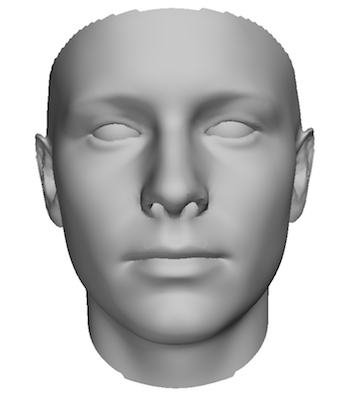
\includegraphics[height=1.15in]{background/images/basel}
		\caption{Basel~\cite{paysan20093d}}\label{fig:db_examples_basel}
	\end{subfigure}
	\begin{subfigure}[b]{0.3\textwidth}
		\centering
		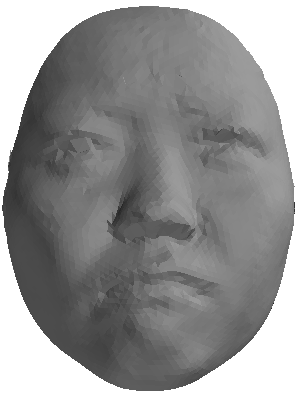
\includegraphics[height=1.2in]{background/images/bu3d}
		\caption{BU3D-FE~\cite{Yin:2006cc}}\label{fig:db_examples_bu3d}
	\end{subfigure}
	\begin{subfigure}[b]{0.3\textwidth}
		\centering
		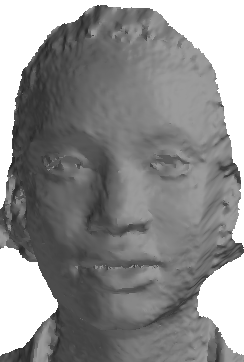
\includegraphics[height=1.2in]{background/images/bp4d}
		\caption{BP4D-S~\cite{Zhang:2014id}}\label{fig:db_examples_bp4d}
	\end{subfigure} \\
	\begin{subfigure}[b]{0.3\textwidth}
		\centering
		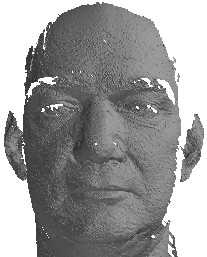
\includegraphics[height=1.2in]{background/images/frgc}
		\caption{FRGC v2~\cite{phillips2005overview}}\label{fig:db_examples_frgc}
	\end{subfigure}
	\begin{subfigure}[b]{0.3\textwidth}
		\centering
		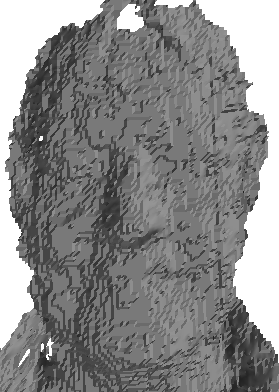
\includegraphics[height=1.2in]{background/images/biwi}
		\caption{BIWI~\cite{fanelli2013random}}\label{fig:db_examples_biwi}
	\end{subfigure}
	\begin{subfigure}[b]{0.32\textwidth}
		\centering
		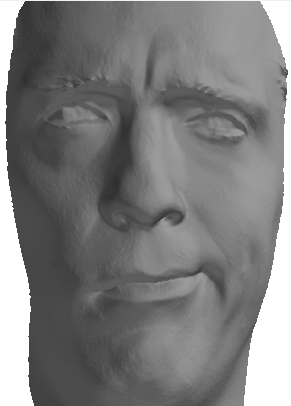
\includegraphics[height=1.15in]{background/images/ict}
		\caption{ICT-3DRFE~\cite{stratou2012exploring}}\label{fig:db_examples_ict}
	\end{subfigure}
	\caption{Examples of the quality of the facial meshes provided in various
	         databases. The meshes were captured by the following systems:
	         \lsubref{fig:db_examples_basel} is from the Basel 3DMM,
	         which was manually cleaned and captured using a structured light
	         scanner, \lsubref{fig:db_examples_bu3d} by the
	         3dMD~\cite{3dmd} active stereo system,
	         \lsubref{fig:db_examples_bp4d} by the
	         Di4D~\cite{di4d} 4D passive stereo system,
	         \lsubref{fig:db_examples_frgc} by the
	         Minolta~\cite{minolta} laser scanning system,
	         \lsubref{fig:db_examples_biwi} by the
	         Microsoft Kinect~\cite{zhang2012microsoft} and
	         \lsubref{fig:db_examples_ict} by a passive stereo
	         light stage~\cite{debevec2000acquiring}.}
\label{fig:db_examples}
\end{figure*}
%%%%%%%%%%%%%%%%%%%%%%%%%%%%%%%%%%%%%%%%
The majority of the databases discussed previously were collected using
commercial apparatus and the focus of the database was the gathering of the
subjects rather than the capturing methodology itself. However, the capturing of
high quality facial surface information is an active area of research and is of
particular interest to the computer graphics community. High quality facial
surface information including mesoscopic details such as fine wrinkles and pores
are necessary for photo-realistic rendering of faces. Photo-realistic rendering
is widely applicable and has seen applications in
films~\cite{borshukov2005universal}, video games~\cite{vonderPahlen:2014kg},
virtual makeup systems~\cite{scherbaum2011computer} and
animatronics~\cite{jung2011believable}. The recovery of these mesoscopic details
requires careful modelling of the interaction between human skin and light. To
this end, many works focus solely on these reflectance characteristics and seek
to provide highly realistic parametric reflectance functions for skin. In this
review, we are only interested in methods that recover realistic 3D shape and
thus do not consider works that focus solely on reflectance function modeling.
For more information about these methods the interested reader should consult
the recent survey on facial appearance capture by \citet{Klehm:2015jb}.

Given the intended use cases for the captured data, facial capturing has focused
on scenarios where both the illumination and camera parameters are tightly
controlled. Thus, the methods considered in this section are not applicable
to the ``in-the-wild'' images that are the focus of this thesis. However,
given that training examples are required to recover reasonable 3D surfaces
from unconstrained images, these training examples provide an upper bound
on the quality of 3D surface that can be recovered. Therefore, it is important
to understand the performance and limitations of the state-of-the-art in
facial capture in order to provide a point of reference for ``in-the-wild''
shape recovery.
%%%%%%%%%%%%%%%%%%%%%%%%%%%%%%%%%%%%%%%%
\begin{table*}
\centering
\begin{adjustbox}{totalheight=\textheight-2\baselineskip,width=\textwidth}
\begin{minipage}{\textwidth}
\centering
\begin{tabular}{@{}llrcccccc@{}}
\toprule
\multicolumn{3}{c}{Method}                                                                       & P-S   & A-S             & SL    & TM-PS   & MS-PS & PC    \\ \midrule
1996                  & \printauthor{Lengagne:1996ej}          &~\cite{Lengagne:1996ej}          & $\cm$ &                 &       &         &       &       \\ \midrule
1999                  & \printauthor{enciso1999synthesis}      &~\cite{enciso1999synthesis}      &       & $\cm$           & $\cm$ & $\cm$   &       &       \\ \midrule
2000                  & \printauthor{debevec2000acquiring}     &~\cite{debevec2000acquiring}     &       &                 & $\cm$ & $\cm$   &       &       \\ \midrule
2001                  & \printauthor{garcia2001low}            &~\cite{garcia2001low}            &       &                 & $\cm$ &         &       &       \\ \midrule
2002                  & \printauthor{d2002modeling}            &~\cite{d2002modeling}            &       & $\cm$           & $\cm$ &         &       &       \\ \midrule
2004                  & \printauthor{zhang2004spacetime}       &~\cite{zhang2004spacetime}       &       & $\cm$           &       &         &       &       \\ \midrule
\multirow{4}{*}{2005} & \printauthor{Leclercq:2005ee}          &~\cite{Leclercq:2005ee}          & $\cm$ &                 &       &         &       &       \\
                      & \printauthor{borshukov2005universal}   &~\cite{borshukov2005universal}   &       & $\cm^{\dagger}$ &       &         &       & $\cm$ \\
                      & \printauthor{nehab2005efficiently}     &~\cite{nehab2005efficiently}     &       & $\cm$           &       & $\cm$   &       &       \\
                      & \printauthor{wenger2005performance}    &~\cite{wenger2005performance}    &       &                 &       & $\cm$   &       &       \\ \midrule
\multirow{2}{*}{2006} & \printauthor{weyrich2006analysis}      &~\cite{weyrich2006analysis}      &       &                 & $\cm$ & $\cm$   &       &       \\
                      & \printauthor{zhang2006high}            &~\cite{zhang2006high}            &       &                 & $\cm$ &         &       &       \\ \midrule
\multirow{4}{*}{2007} & \printauthor{ma2007rapid}              &~\cite{ma2007rapid}              &       &                 &       & $\cm^*$ &       &       \\
                      & \printauthor{bickel2007multi}          &~\cite{bickel2007multi}          &       & $\cm^{\dagger}$ &       &         &       & $\cm$ \\
                      & \printauthor{weise2007fast}            &~\cite{weise2007fast}            & $\cm$ &                 & $\cm$ &         &       &       \\
                      & \printauthor{alexander2009digital}     &~\cite{alexander2009digital}     &       & $\cm$           &       & $\cm^*$ &       &       \\ \midrule
2009                  & \printauthor{furukawa2009dense}        &~\cite{furukawa2009dense}        &       & $\cm^{\dagger}$ &       &         &       & $\cm$ \\ \midrule
\multirow{3}{*}{2010} & \printauthor{Beeler:2010dg}            &~\cite{Beeler:2010dg}            & $\cm$ &                 &       &         &       &       \\
                      & \printauthor{bradley2010high}          &~\cite{bradley2010high}          & $\cm$ &                 &       &         &       &       \\
                      & \printauthor{popa2010globally}         &~\cite{popa2010globally}         & $\cm$ &                 &       &         &       & $\cm$ \\
                      & \printauthor{wilson2010temporal}       &~\cite{wilson2010temporal}       &       &                 &       & $\cm^*$ &       &       \\ \midrule
\multirow{3}{*}{2011} & \printauthor{fyffe2011comprehensive}   &~\cite{fyffe2011comprehensive}   & $\cm$ &                 &       & $\cm^*$ &       &       \\
                      & \printauthor{wu2011high}               &~\cite{wu2011high}               & $\cm$ &                 &       &         &       &       \\
                      & \printauthor{Beeler:2011ey}            &~\cite{Beeler:2011ey}            & $\cm$ &                 &       &         &       & $\cm$ \\
                      & \printauthor{ghosh2011multiview}       &~\cite{ghosh2011multiview}       & $\cm$ &                 &       & $\cm^*$ &       &       \\ \midrule
\multirow{3}{*}{2012} & \printauthor{vogiatzis2012self}        &~\cite{vogiatzis2012self}        &       &                 &       &         & $\cm$ &       \\
                      & \printauthor{valgaerts2012lightweight} &~\cite{valgaerts2012lightweight} & $\cm$ &                 &       &         &       & $\cm$ \\
                      & \printauthor{klaudiny2012high}         &~\cite{klaudiny2012high}         & $\cm$ &                 &       &         & $\cm$ & $\cm$ \\ \midrule
\multirow{2}{*}{2014} & \printauthor{vonderPahlen:2014kg}      &~\cite{vonderPahlen:2014kg}      &       &                 &       & $\cm^*$ &       &       \\
                      & \printauthor{Fyffe:2014hc}             &~\cite{Fyffe:2014hc}             &       &                 &       & $\cm$   & $\cm$ &       \\ \midrule
\multirow{2}{*}{2015} & \printauthor{Gotardo:2015vo}           &~\cite{Gotardo:2015vo}           & $\cm$ &                 &       &         & $\cm$ & $\cm$ \\
                      & \printauthor{graham2015near}           &~\cite{graham2015near}           & $\cm$ &                 &       & $\cm$   &       &       \\ \bottomrule
\end{tabular}
\caption{A timeline of facial capture methods. P-S denotes Passive Stereo,
         A-S is Active Stereo, SL is Structured Light, TM-PS is Time-multiplexed
         Photometric Stereo, MS-PS is Multi-spectral Photometric Stereo and PC
         denotes Performance Capture. \textsuperscript{$\dagger$} denotes marker
         based A-S and \textsuperscript{*} denotes spherical gradient
         illumination.}
\label{tbl:timeline_capture}
\end{minipage}
\end{adjustbox}
\end{table*}
%%%%%%%%%%%%%%%%%%%%%%%%%%%%%%%%%%%%%%%%

The majority of the facial capture literature focuses on two primary areas:
active illumination and
stereo. Passive stereo is a photogrammetric method that requires 2 or more
calibrated cameras who's relative positions are used to infer the 3D position of
an objects surface. A key requirement of passive stereo is a set of
correspondences that are shared across multiple camera views. These
correspondences are defined as a set of 2D coordinates that mark salient areas
of the object, visible across multiple cameras. These 2D points are assumed to
represent the 2D projection of a real 3D point onto each camera plane. It is
these correspondences that are used to form geometric constraints for recovery
of 3D positions. However, the computation of these correspondences is itself
ill-defined as variation in illumination and orientation may cause the
appearance of a true correspondence to vary heavily. Active stereo is an
extension of passive stereo that attempts to simplify the correspondence problem
by projecting a pattern onto the object at capture time. The pattern thus
provides less ambiguous texture cues for computing correspondences. In contrast,
structured light only requires a single camera and unlike active stereo this
camera must be calibrated with respect to the position of the projector
supplying the light pattern. The light patterns projected by the projector
encode the correspondences and 3D information is recovered via triangulation.
Active illumination methods such as
Photometric Stereo (PS)~\cite{woodham1980photometric} uses reflectance
information in order to recover surface information. In traditional photometric
stereo a number of images are captured under different know illumination
conditions and these are used to recover surface normals for the objects in the
image. For and in-depth discussion of PS methods please see
\cref{sec:bg_ps}.

\textbf{Passive (computational) stereo} is an extremely common technique for
surface recovery and the geometric relationships between two calibrated cameras
are relatively well
understood~\cite{barnard1982computational,seitz2006comparison}. When passive
stereo is applied to reasonably smooth, convex objects in uncluttered scenes, as
is generally the case when capturing faces, it is largely considered a
technology. Commercial systems such as 3dMD~\cite{3dmd} and Di4D~\cite{di4d} are
employed in many areas of entertainment and have been used to capture many of
the high quality databases in \cref{tbl:timeline_db}. Both of these companies
also provided high frame rate systems that are capable of capturing 3D
information at 60+ fps, albeit temporally consistent meshes still require
further post-processing. For this reason, few works in passive stereo focus
solely on the recovery of macroscopic shape using only stereo. Whilst older
works such as that of \citet{Lengagne:1996ej} required 3D models to perform
inference, such as segmentation, on depth maps, modern depth maps are of much
higher quality. Even relatively recent reviews on the subject of passive stereo
applied to faces~\cite{Leclercq:2005ee} have become obsolete given the price and
quality of modern digital camera systems. For example, the work of
\citet{Beeler:2010dg} demonstrates that standard passive stereo methods can
recover 3D surfaces that contain high frequency features such as wrinkles.
The highest quality result presented by \citet{Beeler:2010dg} comes from a seven
camera studio setup where per-pixel correspondences and disparity map refinement
is computed in a coarse-to-fine manner. Further constraints are imposed that are
face specific including a smoothness constraint when computing correspondences
and a second-order anisotropic surface consistency term that reduces smoothing
across depth discontinuities in the disparity maps. Finally, mesoscopic details
are transferred into the mesh via a photometrically consistent surface
refinement procedure. Although the recovered details are not metrically correct,
they do significantly improve the qualitative accuracy of the recovered surface.
Under the assumption that these mesoscopic variations in intensity are linked to
variations in the geometry of the skin, a high-pass filter is first performed in
order to filter out any details captured by stereo. Then, the result of the
stereo is refined along the surface normal direction and is weighted to ignore
high frequency areas caused by larger features such as hairs.
\citet{bradley2010high} propose a passive method for performance capture that
focuses on the concept that modern cameras are capable of capturing such high
detail that stereo-matching is greatly simplified. Fourteen stereo cameras, in
seven pairs, are focused on seven overlapping facial regions, allowing the
capture of high frequency facial detail such as pores. This high frequency
detail is utilised for stereo matching and the seven overlapping regions are
then merged to recover a single high quality mesh. The remainder of the work
focuses on recovering a topologically consistent mesh throughout the sequence by
applying optical flow and drift correction methods. The output is a performance
capture sequence at 30 FPS with a high resolution mesh and texture map
with consistent topology across the sequence.
\citet{wu2011high} propose to augment a standard passive stereo result with
a term to enforce photometric consistency. However, they optimise in the space
of the image gradients rather than directly perturbing the surface by the
recovered spherical harmonic orientations, as is done
in~\cite{nehab2005efficiently}.

\textbf{Active stereo} augments traditional passive stereo with a signal that is
used to aid in the stereo correspondence step. Typically, this signal is a laser
or light that is shone on the subjects faces in order to give consistent
features where matching may be difficult such as the smooth low texture areas of
the face (e.g cheeks). For example, \citet{enciso1999synthesis} proposed a noisy
shape pattern to aid in stereo reconstruction whereby the result is registered
with a generic mesh for use in animation. Similarly, \citet{d2002modeling}
use a random noise pattern in order to aid in stereo matching and allow
for extremely efficient depth generation.
\citet{zhang2004spacetime} used the
Spacetime Stereo~\cite{zhang2003spacetime,davis2005spacetime} technique to
recover a 3D mesh per frame. A set of striped lighting patterns are projected
across the face, with every third frame having no projection in order to recover
texture. These textured frames are use for optical flow a single topologically
consistent template mesh is deformed to be photometrically consistent with the
frame.
Although active stereo is typically defined in terms of improving stereo
matching via light projection, early marker based stereo methods can also be
seen as methods for improving stereo matching.
Stemming back to the work of \citet{williams1990performance}, manually placing
markers on faces became the de facto method for performance
capture~\cite{bickel2007multi,furukawa2009dense,bredow2005mocap},
used in films such as \textit{The Polar Express (2004)},
\textit{Dawn of the Planet of the Apes (2014)} and
\textit{The Lord of the Rings: The Two Towers (2002)}.
\citet{bickel2007multi} used painted markers to map deformations from two
different resolution camera pairs and used these markers to drive the
deformations of a previously recorded high resolution mesh.
\citet{furukawa2009dense} used densely painted black markers to perform
scene flow form stereo. Initialised in the first frame with a reconstruction
provided by \citet{Furu:2010:PMVS}, patch-based scene flow is computed across
the sequence in order to maintain a single mesh topology.

\textbf{Structured light} methods drop the requirement of a second camera in
favour of a calibrated light projector. When a known lighting pattern, even as
simple as a grid~\cite{will1971grid}, is projected onto the scene it becomes
possible to estimate the surface by measuring the distortion of the light by the
surface. For example, the work of \citet{garcia2001low} provided a method
for full 3D surface recovery by performing structured light across multiple
head poses and then merging them into a final result.
Structured lights is particularly effective for real-time
acquisition~\cite{rusinkiewicz2002real} and more recently was used by the
Microsoft Kinect~\cite{zhang2012microsoft}. Although the quality of output, as
depicted for the BIWI head pose database in
\cref{fig:db_examples_biwi}, is known to be low in the case of the Microsoft
Kinect, structured light is capable of high recovering high quality macroscopic
shape. In fact, recent work has shown that by using specially crafted
homogeneous codes for structured lighting it is possible to recover light
transport information even under strong ambient lighting.
By synchronising a laser projector with the rolling shutter of the camera and
masking out pixels that do not lie on the projector-camera epipolar plane it
becomes possible to only receive light from the laser within the epipolar plane.
This means that very little ambient light pollutes the laser emitted
signal and it becomes possible to measure the structured lighting pattern
even within bright scenes such as outdoors~\cite{o2015homogeneous}.
Real time capture of high-quality facial shape using
structured light has been proposed by \citet{zhang2006high,weise2007fast}.
\citet{zhang2006high,wang2004high} proposed a set of custom hardware that
enabled up to 120 fps capture and reconstruction. The reconstruction is computed
rapidly via a novel three-step sinusoidal phase shifting algorithm.
\citet{zhang2006high} proceed to non-rigidly align a generic model to the output
meshes in order to achieve a topologically consistent sequence.
\citet{weise2007fast} also utilise a projected light pattern, but in contrast to
\citet{zhang2006high}, the projector is calibrated with respect to two stereo
cameras and so extra constraints are imposed on stereo matching. This has the
advantage that the structured lighting constraints complement the stereo
matching, but due to the phase shifted structure of the lighting patterns three
consecutive images are required for 3D recovery. Thus, motion artifacts become
evident in a dynamic scene. To mitigate this, \citet{weise2007fast} propose a
motion compensation scheme involving estimating the phase error cause by motion.

\textbf{Active illumination} is a general term that we are using to describe
methods that attempt to recover surface information by using structured
illumination patterns. In contrast to active stereo and structured
light, these illumination patterns are not designed to encode geometric
information. Instead, the illumination is designed to reveal surface information
that may not be visible to traditional stereo methods.
The most commonly employed surface recovery
algorithm is PS~\cite{woodham1980photometric}, which is discussed in detail in
\cref{sec:bg_ps}. The use of PS for high quality facial capture
can be separated into two distinct categories: time-multiplexing~\cite{ma2007rapid,%
fyffe2011comprehensive,alexander2009digital,vonderPahlen:2014kg,%
malzbender2006surface,wilson2010temporal,ghosh2011multiview} and
multi-spectral~\cite{vogiatzis2012self,brostow2011video,fyffe2011single}.

\textit{Time multiplexed PS} involves taking multiple images, each under
a different illumination, over a short time-frame. Although databases such as
YaleB~\cite{georghiades2001fromfew} and Photoface~\cite{zafeiriou2013photoface} were produced
using time multiplexed PS, modern high quality capturing using PS employs
many lights generally arrayed in a ``light-stage''. One of the earliest works
using a light-stage for facial capture was the work of
\citet{debevec2000acquiring}, which focused on extrapolating a reflectance
field from a human face. Here, two cameras record the subject and a spotlight
suspended 1.5 metres away from the subject is revolved at approximately 25 RPM,
producing around 2048 output images. Both subsurface (diffuse) and specular data
were recovered using chromaticity analysis and the specular component was
utilised to allow relighting from novel viewpoints. This work focused on the
recovery of reflectance information for image relighting and required
approximately one minute for capture, making it impractical for dynamic use.
\citet{weyrich2006analysis} provided a more
detailed reflectance field by proposing a novel skin reflectance model
that can be parametrised from measurements. They also use a light-stage and
capture 150 fixed illumination patterns across 16 cameras to allow for more
accurate specular normal estimation. They also measure skin translucency
using a fibre optic spectrometer~\cite{nickell2000anisotropy} and provide
a reflectance model built from 149 subjects that is diverse across race, age and
gender. Both \citet{weyrich2006analysis} and \citet{debevec2000acquiring} used
a structured light method to recover
the macroscopic shape and then augmented this model with the normals
recovered from the illumination~\cite{nehab2005efficiently}.
\cite{nehab2005efficiently} provide an efficient method for combining coarse
surface estimates with normal information. In particular, they demonstrate the
efficiency of their method with data capture using an
active stereo method~\cite{zhang2003spacetime,davis2005spacetime} which is
augmented with surface normals recovered from time-multiplexed photometric
stereo.
\citet{wenger2005performance} utilised a light-stage in order to capture
short performances. A high speed camera and time multiplexed illumination was
utilised to capture many images. They also experimented with different
illumination bases to attempt to improve the lighting of the subject
under such short exposures. Diffuse normals are recovered with PS and
reflectance mapping~\cite{miller1984illumination} is utilised for facial
relighting.
\citet{malzbender2006surface} also propose PS for dynamic
capture and provide a hardware set up that enables real-time capture
of reflectance information of small objects. However, specular effects
were not considered.
To improve the performance of multi-illumination time multiplexed
capture, \citet{ma2007rapid} propose a spherical gradient illumination pattern.
Only four spherical gradient illumination patterns are required to allow
normal estimation from arbitrary viewpoints. A light-stage consisting of 156
LED lights and a single camera are used to construct the 4 illumination
patterns. The primary novelty, other than arbitrary viewpoint synthesis, is
the simple separation of diffuse and specular normals by polarisation of the
gradients. Due to the lower number of lighting configurations required,
\citet{ma2007rapid} do not require a high speed camera.
\citet{wilson2010temporal} extend the work of \citet{ma2007rapid} to
improve the temporal resolution of the capturing without resorting to
high-speed cameras. In order to model the non-rigid movement present
during a facial performance, \citet{wilson2010temporal} perform optical
flow to ensure alignment. However, most optical flow algorithms will fail under
the large illumination variation present in the gradient illuminated images.
Therefore, \citet{wilson2010temporal} augment the 4 spherical gradient
illumination patterns ($x$, $y$, $z$, $0$) with the inverse spherical
gradient patterns ($x$, $-x$, $y$, $-y$, $z$, $-z$, $0$), where $0$ is the
fully illuminated frontal image. They note that the summation of two
complementary gradient pairs cancel out and yield the fully lit image. Thus
optical flow can be computed between complementary gradient pairs and the fully
lit image with any existing optical flow algorithm, assuming moderate dynamic
movement. Similar to~\cite{ma2007rapid,debevec2000acquiring,weyrich2006analysis},
\citet{wilson2010temporal} augment the output of a coarse model, predicted
from passive stereo, with their recovered normals.
\citet{fyffe2011comprehensive} extend the work of \citet{wilson2010temporal}
with multiple stereo viewpoints that are merged into a single output mesh.
They also propose a maximum likelihood estimate of the output shape
that fuses the coarse geometry estimate from stereo with photometric normals
to provide a unified method for recovering stereo fused with normals.
\citet{ghosh2011multiview} note that although \citet{fyffe2011comprehensive}
performed multi-view reconstruction, there were unable to apply polarisation
in order to recover diffuse and specular normals. Therefore,
\citet{ghosh2011multiview} propose a new set of spherical gradient
illumination patterns that allow view independent polarisation
for viewpoints that lie along the yaw plane (profile-to-profile). Like
\citet{fyffe2011comprehensive}, they perform geometry recover jointly
on the stereo and normals estimates, however, they do not merge the multiple
views and instead recover a single displacement map. Most recently,
\citet{graham2015near} have proposed a fast capture method involving 24 cameras
and six ring lights where each flash is fired sequentially with a subset
of the cameras. Thus, 24 specular reflection angles are recovered which
enables chromaticity separation of the diffuse and specular normals. Passive
stereo is performed to recover a base mesh and diffuse and specular normals
are separated using the chroma-space of \citet{zickler2008color}. A modified
PS algorithm is performed to recover the diffuse and specular normals and
the passive stereo mesh is augmented with the diffuse normals followed
by the specular normals~\cite{nehab2005efficiently}.

\textit{Multi-spectral PS} involves illuminating an object under
multiple constant illuminations that are spectrally separable. Unlike
time-multiplexed methods, spectral methods do not require multiple images
and thus have the advantage that optical flow or other alignment assumptions
are not required. However, the difficulty lies in effectively separating the
illumination channels in order perform surface recovery. To this end
Hern{\'a}ndez and co-authors have a number of works that provide
calibration methods~\cite{vogiatzis2012self,hernandez2008multiview,brostow2011video}
for colour PS~\cite{drew1992shape}. The most relevant work of Hern{\'a}ndez
is the work of \citet{vogiatzis2012self}, which proposes a self-calibrating
method for multi-spectral 3D face capture. A rigid motion is performed by
the subject and structure-from-motion is used to recover approximate camera
parameters. Passive stereo is then performed to recover an initial dense
shape estimate and this is then used to calibrate the multi-spectral PS.\@
Once calibrated, the method of \citet{brostow2011video} can be used to
recover non-rigid PS from multi-spectral illumination.
\citet{fyffe2011single} generalise the typical 3-colour multi-spectral
and provide a practical 6-channel capture system. A beam splitter is used
to obtain 6-channel photographs via 2 cameras that are filtered using
2 different dichroic filters that separate the visible light spectrum
into 6 non-overlapping bands. Calibration is performed manually using colour
charts.

\textbf{Performance Capture.} Furthering the efforts on capturing high
quality static geometry and reflectance information, there have also been
a number of works that focus on performance capture. Performance capture places
constraints on the capture methodology as it becomes necessary to achieve
a frame-rate that is sufficient for non-rigid deformation recording.
Furthermore, it may also be desirable to recover a facial surface with
consistent topology across all frames. Whilst this may be handled during
post-processing of the capture, it is often more accurate to enforce
the consistent topology during geometry recovery. \citet{bickel2007multi}
utilise painted face markers for sparse motion capture recording. A dense
generic facial template is then deformed using the motion capture displacements
and wrinkles are synthesised from the texture information to recover
``medium-scale'' details. \citet{popa2010globally} record a sequence by
employing the method of \citet{bradley2010high}. A hierarchical sequence
is then built by pairing consecutively longer sub-sequences together. Sparse
optical flow is employed as a set of soft correspondences and a patch-based
optimisation method is employed to build a single topologically consistent
mesh. \citet{Beeler:2011ey} extend their earlier work~\cite{Beeler:2010dg}
to recover a single mesh from a sequence. They employ the notion
of ``anchor frames'' to partition a sequence whereby optical flow is applied
in order to track deformations between anchor frames. These deformations
are then propagated onto a manually identified reference frame and a further
refinement process is employed to introduce spatial and temporal consistency.
\citet{valgaerts2012lightweight} propose to use binocular passive stereo
in order track a coarse person specific template over the sequence. They
propose a novel image based scene flow method to deform the template
mesh in a photometrically consistent manner across the sequence. This coarse
geometry is then refined using a novel shading energy that is similar
but more efficient than the one proposed in \citet{wu2011high}.
\citet{klaudiny2012high} also propose to augment the result of passive
stereo with shading information. They introduce multi-spectral PS in
conjunction with passive stereo in order to recover higher frequency
shading related features. A consistent topology is recovered using
a on-sequential spanning tree. However, uniform white make-up must be applied
to the actors face in order to allow multi-spectral calibration. Similarly,
\citet{Gotardo:2015vo} propose a hybrid method that attempts to iteratively
recover a high quality performance capture result by utilising both
passive stereo and multi-spectral PS information. They perform
correspondence recovery over small windows and geometry information is thus
recovered using stereo. This coarse geometry is refined using multi-spectral PS
and then illumination normalised albedo maps are synthesised using the surface
normal information. These albedo images are then re-utilised for optical flow
computation to iteratively improve the initial stereo recovery.
\citet{Fyffe:2014hc} employ the capturing system of \citet{ghosh2011multiview}
to recover a base set of person specific meshes. A uniformly lit
sequence is then captured in stereo and a ``performance flow graph'' is
computed whereby optical flow is calculated between every pair of frames.
An optimisation procedure is proposed to perform 3D tracking between the
static scans and the performance capture is parameterised between the given
static 3D scans a single artist rigged neutral mesh.
%%%%%%%%%%%%%%%%%%%%%%%%%%%%%%%%%%%%%%%%%%%%%%%%%%%%%%%%%%%%%%%%%%%%%%%%%%%%%%%%

%%%%%%%%%%%%%%%%%%%%%%%%%%%%%%%%%%%%%%%%%%%%%%%%%%%%%%%%%%%%%%%%%%%%%%%%%%%%%%%%
\section{Shape-from-Shading}\label{sec:bg_sfs}
%%%%%%%%%%%%%%%%%%%%%%%%%%%%%%%%%%%%%%%%%%%%%%%%%%%%%%%%%%%%%%%%%%%%%%%%%%%%%%%%
%%%%%%%%%%%%%%%%%%%%%%%%%%%%%%%%%%%%%%%%
\begin{figure*}[t]
	\centering
	\begin{subfigure}[b]{0.24\textwidth}
		\centering
		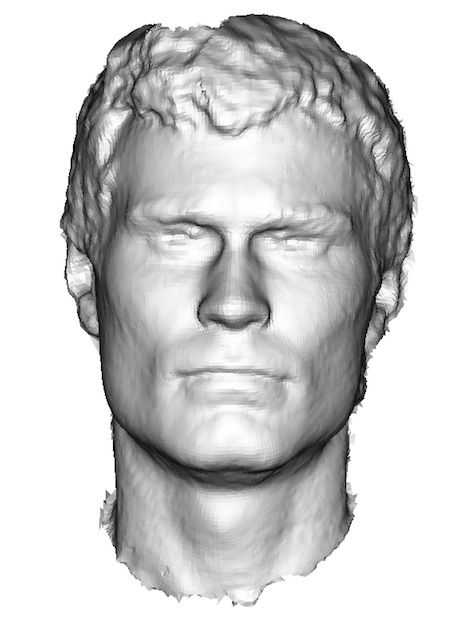
\includegraphics[height=2in]{background/images/frontal}
		\caption*{Frontal}
	\end{subfigure}
	\begin{subfigure}[b]{0.24\textwidth}
		\centering
		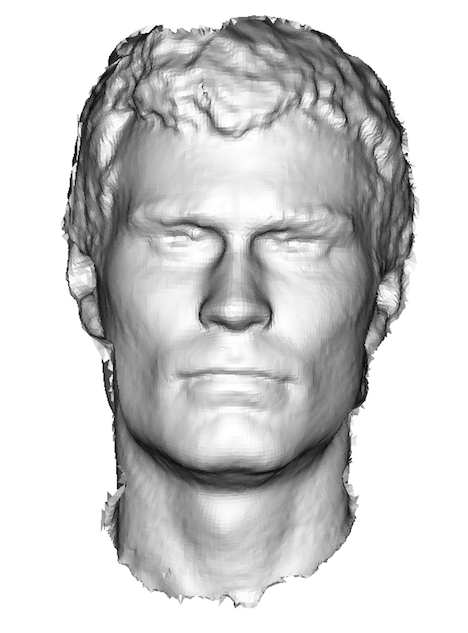
\includegraphics[height=2in]{background/images/invert}
		\caption*{Inverted}
	\end{subfigure}
	\begin{subfigure}[b]{0.24\textwidth}
		\centering
		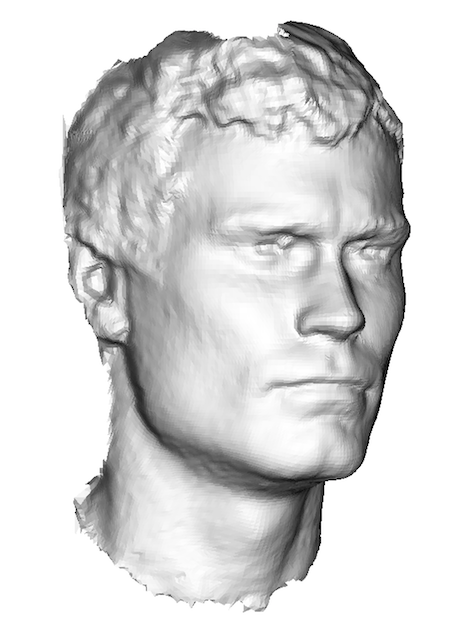
\includegraphics[height=2in]{background/images/frontal_rotate}
		\caption*{Frontal}
	\end{subfigure}
	\begin{subfigure}[b]{0.24\textwidth}
		\centering
		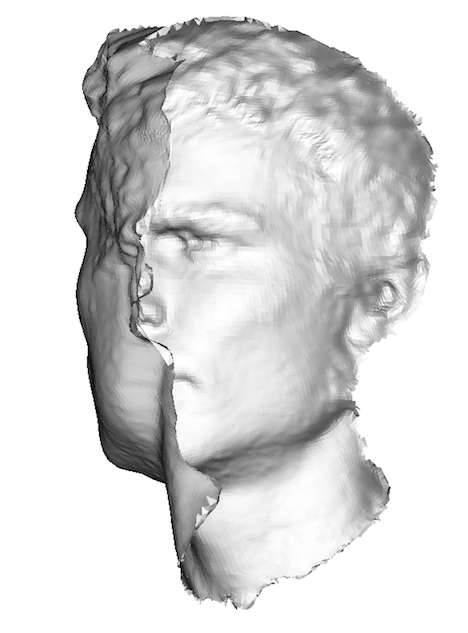
\includegraphics[height=2in]{background/images/invert_rotate}
		\caption*{Inverted}
	\end{subfigure}
	\caption{An example of a bas-relief ambiguity for a mesh illuminated
	         frontally under orthographic projection, with a lambertian shader.
	         ``Inverted'' implies that the mesh is actually facing away from the
	         camera and thus the interior is visible, as demonstrated by the
	         rotated ``Inverted'' image. Both of the non-frontal images are
	         rotated versions of the frontal images, approximately $25^\circ$
	         around the Yaw axis.}
\label{fig:bg_sfs_bas_relief}
\end{figure*}
%%%%%%%%%%%%%%%%%%%%%%%%%%%%%%%%%%%%%%%%
Shape-from-shading (SfS)~\cite{horn1970shape} is the process of attempting to
recover surface information from an object in an image using \textit{inverse
rendering}, or \textit{image formation}, methods. The primary assumption is that
shading, or the intensity of a pixel in the image, is generated as a function of
the surface geometry and its interaction with light reflected/absorbed by the
surface and captured by an imaging device. Naturally, the reality of this
process in the physical world is a complex interaction between light and both
microscopic and macroscopic elements of the surface structure. This is further
complicated by the noise present in the recording procedure of the camera
sensing hardware. Furthermore, it is well known that shading alone is
insufficient to disambiguate shape. For example, the well known bas-relief
ambiguity~\cite{belhumeur1999bas} is demonstrated for a facial mesh in
\cref{fig:bg_sfs_bas_relief}. The bas-relief ambiguity states that for an object
imaged under orthographic projection that exhibits Lambertian reflectance, there
exists a family of transformations (generalized bas-relief transformations) for
which the images produced will be identical. In fact, more generally there
exists an infinite number of ways to describe any image given only shading
information through different arrangements of surfaces, lightings and
albedos~\cite{adelson1996perception}. However, despite the ill-posedness of the
SfS problem, shading does in fact provide a very strong imaging prior and many
higher frequency detail such as wrinkles can only be recovered using shading
cues. Before discussing the facial surface recovery literature, we briefly
describe the image formation problem including the common assumptions
made.
%%%%%%%%%%%%%%%%%%%%%%%%%%%%%%%%%%%%%%%%%%%%%%%%%%%%%%%%%%%%%%%%%%%%%%%%%%%%%%%%
\subsection{Image Formation}
%%%%%%%%%%%%%%%%%%%%%%%%%%%%%%%%%%%%%%%%%%%%%%%%%%%%%%%%%%%%%%%%%%%%%%%%%%%%%%%%
%%%%%%%%%%%%%%%%%%%%%%%%%%%%%%%%%%%%%%%%
\begin{figure*}[t]
	\centering
	\begin{tabular}{cc}
		\multicolumn{2}{c}{
			\begin{subfigure}[b]{\textwidth}
				\centering
				\caption*{Radiometric Terms}
				\begin{tabular}{@{}lll@{}}
					\toprule
					Term              & Symbol                                      & Unit                 \\ \midrule
					Solid Angle       & $d\omega$                                    & ${sr}^{-1}$          \\
					Radiant Flux      & $\Phi$                                       & $W$                  \\
					Radiant Intensity & $J = d \Phi / d \omega$                      & $W {sr}^{-1}$        \\
					Irradiance        & $E = d \Phi / d A$                           & $W m^{-2}$           \\
					Radiance          & $L = d^2 \Phi / (dA \cos{\theta_r} d\omega)$ & $W m^{-2} {sr}^{-1}$ \\ \bottomrule
				\end{tabular}
			\end{subfigure}
		} \\[2cm]
		\begin{subfigure}[b]{0.48\textwidth}
			\centering
			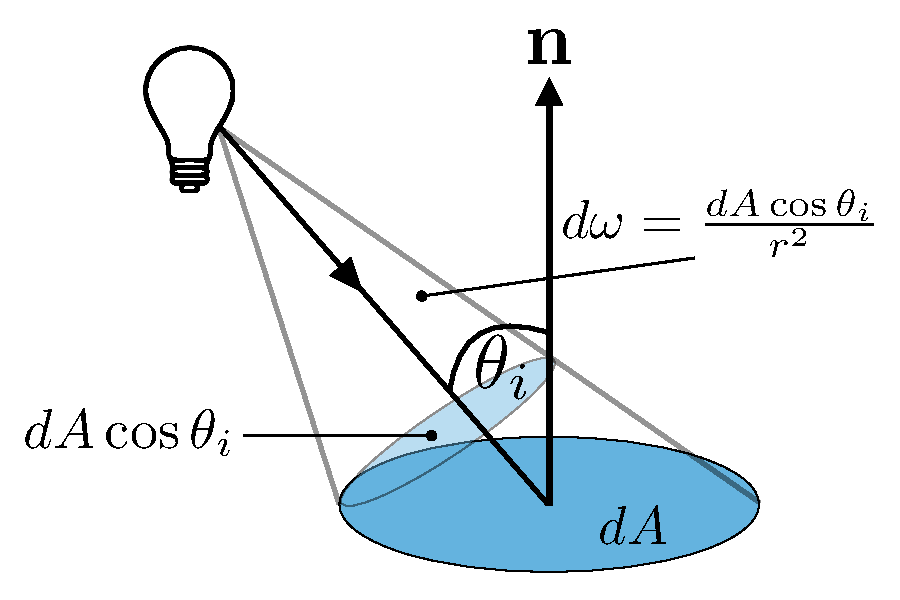
\includegraphics[width=\textwidth]{background/images/irradiance}
			\caption*{Irradiance}
		\end{subfigure} &
		\begin{subfigure}[b]{0.48\textwidth}
			\centering
			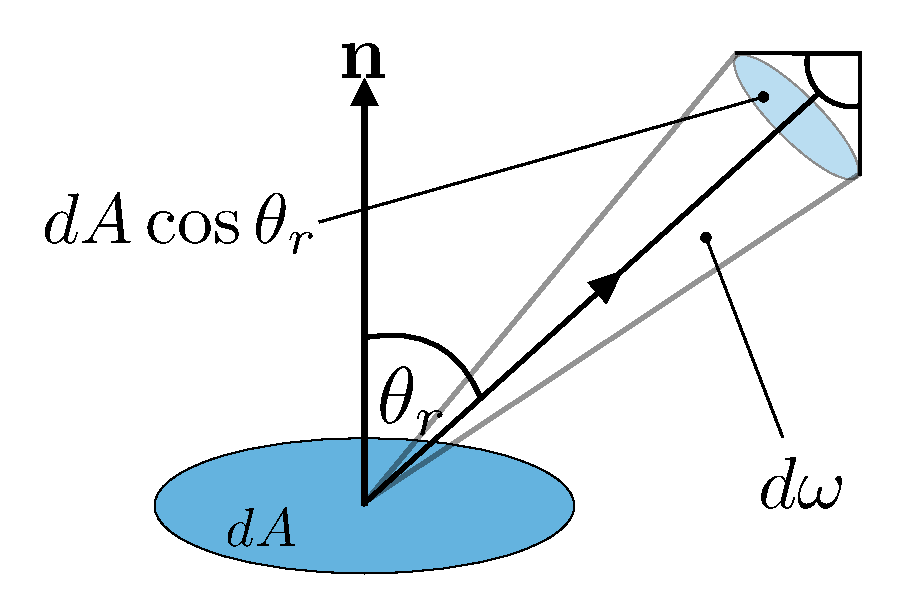
\includegraphics[width=\textwidth]{background/images/radiance}
			\caption*{Radiance}
		\end{subfigure}
	\end{tabular}
	\caption{Illustration of common radiometric terms, focusing on the surface
	         irradiance and radiance. ${sr}^{-1}$ denotes steradians, the
	         Standard International unit of solid angular measure and
	         $W$ denotes watts.}
\label{fig:bg_sfs_rad_irrad}
\end{figure*}
%%%%%%%%%%%%%%%%%%%%%%%%%%%%%%%%%%%%%%%%
%TODO: Need a section on Spherical Harmonics
When discussing image formation methods a number of assumptions are commonly
made in order to ensure tractability of of the rendering physics. Firstly,
unless explicitly mentioned, we assume an orthographic camera projection. This
is a reasonable assumption for most facial images as faces tend to the be
the focus of an image and thus photographs are commonly taken close enough
to the face that perspective effects are minimal. We also only consider
reflection functions that can be expressed as a Bidirectional
Reflectance-Distribution Function (BRDF). A BRDF is a convenient construct
that allows the expression of how bright a surface will appear from a given
view point direction when illuminated from another direction. More formally, it
is the ratio of the reflected radiance in the viewing direction to the
irradiance, in the direction toward the light source.
See \cref{fig:bg_sfs_rad_irrad} for an illustration of the radiance and
irradiance as well as a table of useful radiometric terms. BRDFs are functions
of local illumination and do not model global illumination effects such
as shadows or inter-reflections.
\textit{Radiant flux} is the power emitted from a light source, measured in
watts $(W)$.
The \textit{solid angle} subtended by a surface patch is defined as the
surface area of a unit sphere covered by the surface's projection onto the
sphere and is measured in steradians $(sr)$. In \cref{fig:bg_sfs_rad_irrad},
$r$ refers to the distance from the sphere's origin to the patch.
\textit{Radiant intensity} is the radiant flux per unit solid angle and is
measured in watts per steradian $(W {sr}^{-1})$.
The \textit{irradiance} is the amount of energy received by a given surface
patch, measured in watts per square meter $(W m^{-2})$.
The \textit{radiance} is the amount of energy emitted per unit foreshortened
surface area per unit solid angle, measured in watts per square meter
per steradian $(W m^{-2} {sr}^{-1})$. In \cref{fig:bg_sfs_rad_irrad},
the unit foreshortened area is given by $dA \cos{\theta_r}$.
It is important to note that radiance, unlike irradiance, is a directional
quantity. This implies that the viewing angle affects the amount of perceived
light from a given image area and for some reflectance functions that manifests
as specular style highlights. Finally, we rely on the fact that the image
irradiance captured by the camera sensor is directly proportional to the
scene radiance~\cite{horn1979calculating}. To simplify matters, when referring
to image irradiance we assume that the linear relationship between the scene
radiance and image irradiance is the identity
\ie~scene radiance = image irradiance. An illustration of the relationship
between scene radiance and image irradiance is given in
\cref{fig:bg_sfs_scene_to_intensity}.

Given the previous definitions, we can now formally define the general equation
for a BRDF
%%%%%%%%%%%%%%%%%%%
\begin{align}\label{eg:bg_sfs_general_brdf}
	f(\theta_i,\phi_i;\theta_r,\phi_r) &= \frac{L(\theta_r,\phi_r)}{E(\theta_i,\phi_i)} \\
	L(\theta_r,\phi_r)                 &= E(\theta_i,\phi_i) f(\theta_i,\phi_i;\theta_r,\phi_r) \\
	L(\theta_r,\phi_r)                 &= \int_{2\pi} I_{\operatorname{src}}(\theta_i,\phi_i) f(\theta_i,\phi_i;\theta_r,\phi_r) \; \cos{\theta_i} \; d\omega_i,
\end{align}
%%%%%%%%%%%%%%%%%%%
where $I_{\operatorname{src}}(\theta_i,\phi_i)$ is the intensity of output
from a given light source. In fact, assuming isotropy, the BRDF is
only a function of 3 parameters, $f(\theta_i,\theta_r, \Delta \phi)$ where
$\Delta \phi = \phi_i - \phi_r$. An isotropic BRDF is invariant to rotations
around the direction of the normal. We also assume Helmholtz reciprocity, which
states that if the light source and viewing direction are swapped the BRDF
remains unchanged
\ie~$f(\theta_i,\phi_i;\theta_r,\phi_r) = f(\theta_r,\phi_r;\theta_i,\phi_i)$.
An illustration of the general BRDF is given in \cref{fig:bg_sfs_brdf_example}.
%%%%%%%%%%%%%%%%%%%%%%%%%%%%%%%%%%%%%%%%
\begin{figure*}[t]
	\centering
	\begin{subfigure}[b]{0.45\textwidth}
		\centering
		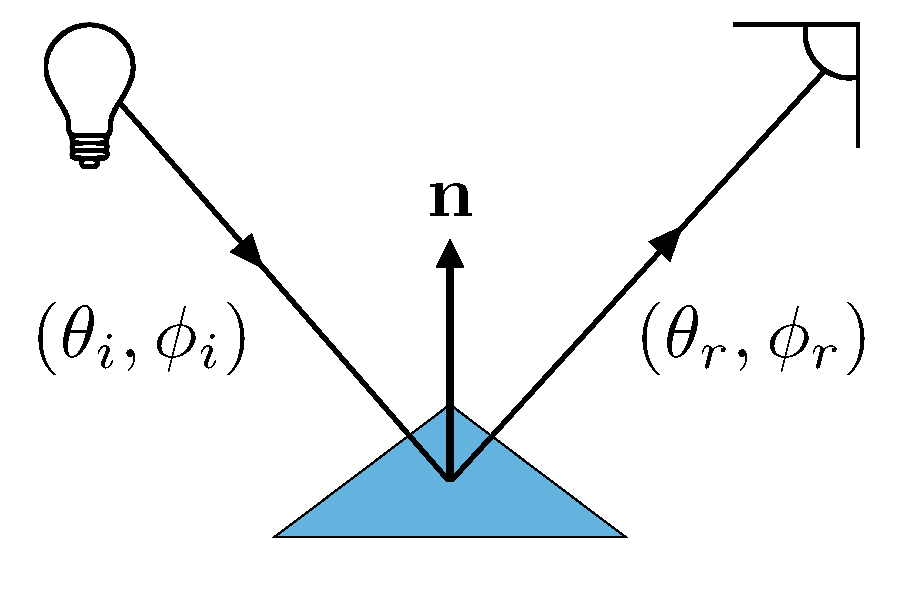
\includegraphics[width=\textwidth]{background/images/general_brdf}
		\caption*{General BRDF}
	\end{subfigure}
	\begin{subfigure}[b]{0.45\textwidth}
		\centering
		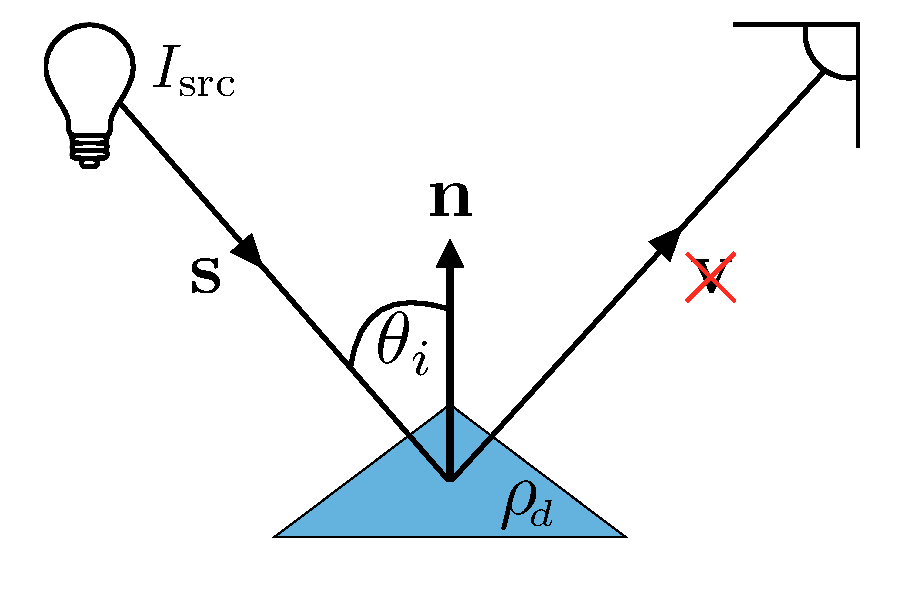
\includegraphics[width=\textwidth]{background/images/lambertian_brdf}
		\caption*{Lambertian BRDF}
	\end{subfigure}
	\caption{The left image shows the general radiance equation for a generic
	         BRDF that is parametrized by the irradiance $(\theta_i, \phi_i)$
	         and radiance $(\theta_r, \theta_r)$ reflecting from the surface.
	         The right image shows the Lambertian BRDF assuming unit light
	         intensity. Note that the Lambertian BRDF is independent of
	         the viewing direction.}
\label{fig:bg_sfs_brdf_example}
\end{figure*}
%%%%%%%%%%%%%%%%%%%%%%%%%%%%%%%%%%%%%%%%

The most commonly assumed BRDF is that of the Lambertian BRDF.\@ A Lambertian
BRDF models only the diffuse component of radiance and is physically accurate
for materials whose reflectance are dominated by scattering effects. For
example, a commonly cited highly Lambertian object is chalk. In more
detail, the Lambertian BRDF modifies \cref{eg:bg_sfs_general_brdf} such that
$f(\theta_i,\theta_r, \Delta \phi) = \rho_{\smallsub{d}} / \pi$ and therefore
the image irradiance is defined as
%%%%%%%%%%%%%%%%%%%
\begin{equation}\label{eg:bg_sfs_lambertian_brdf}
	L_{\operatorname{lambert}} = I_{\operatorname{src}} \frac{\rho_{\smallsub{d}}}{\pi} \cos{\theta_i} =
	I_{\operatorname{src}} \frac{\rho_{\smallsub{d}}}{\pi} \bb{n}^T \bb{s},
\end{equation}
%%%%%%%%%%%%%%%%%%%
where $\bb{n} = {[n_x, n_y, n_z]}^T \in \R^{3}$ is the unit normal of the surface patch,
$\bb{s} = {[s_1, s_2, s_3]}^T \in \R^{3}$ is the unit
light vector and $\rho_{\smallsub{d}}$ is the diffuse albedo scaled by $1/\pi$
to ensure $\rho_{\smallsub{d}} \in [0, 1]$. The Lambertian BRDF is illustrated
in \cref{fig:bg_sfs_brdf_example}. Note that for the Lambertian BRDF, the image
irradiance does not depend on the viewing direction and thus
$L_{\operatorname{lambert}}$ is not a function of $(\theta_r,\phi_r)$.
Physically, this implies that Lambertian surfaces do not exhibit specular
effects and appear evenly lit from all viewing angles, scaled by the cosine
of the angle between the light and normal vectors. Commonly,
\cref{eg:bg_sfs_lambertian_brdf} is simplified further as it is assumed that the
radiant intensity is normalised and thus the most commonly cited form of the
Lambertian BRDF is
%%%%%%%%%%%%%%%%%%%
\begin{align}\label{eg:bg_sfs_lambertian_simple}
	L_{\operatorname{lambert}} = \rho_{\smallsub{d}} \bb{n}^T \bb{s},
\end{align}
%%%%%%%%%%%%%%%%%%%
Finally, \cref{eg:bg_sfs_lambertian_simple} may generate outputs that are
not physically realisable. For example, a patch lit from the vector opposite
its normal would produce negative intensity. Therefore, the correct physical
form of the Lambertian BRDF is
$L_{\operatorname{lambert}} = \rho_{\smallsub{d}} \max(\bb{n}^T \bb{s}, 0)$.
For completeness, is it worthwhile noting that the image irradiance, formed
through the interaction of the scene radiance and the optic lens, is not
the final measured pixel intensity value commonly utilized on Computer Vision.
The final measured pixel intensity is a function of the image irradiance
and a non-linear function commonly referred to as the
\textit{camera response function}. The camera response function models a number
of effects such as detector sensitivity, vignetting, lens falloff and the
camera electronics. In fact, many manufacturers intentionally model
the camera response function to simulate the responses of other media
such as film~\cite{grossberg2003space}. The calibration function is consistent
over the entire image area and is invertible. Therefore, the camera response
function modifies the image irradiance as follows: $I = f(L)$ where $I$ denotes
a singe pixel in the image, $f$ denotes the camera response function and $L$
denotes the image irradiance as was being discussed above.
\cref{fig:bg_sfs_scene_to_intensity} gives an illustration of this process. Note
that the transformation from scene radiance to image irradiance is
linear~\cite{horn1979calculating} and was previously ignored when discussing
radiometric terms. Camera response calibration requires acquiring controlled
images of a MacBeth board or other colour chart, or the use of pre-calculated
response model~\cite{grossberg2003space}. Therefore, unless explicitly
mentioned, we make the strong assumption that the camera response function
is the identity function and thus pixels in any given image directly
represent the scene radiance.
%%%%%%%%%%%%%%%%%%%%%%%%%%%%%%%%%%%%%%%%
\begin{figure}[t]
	\centering
	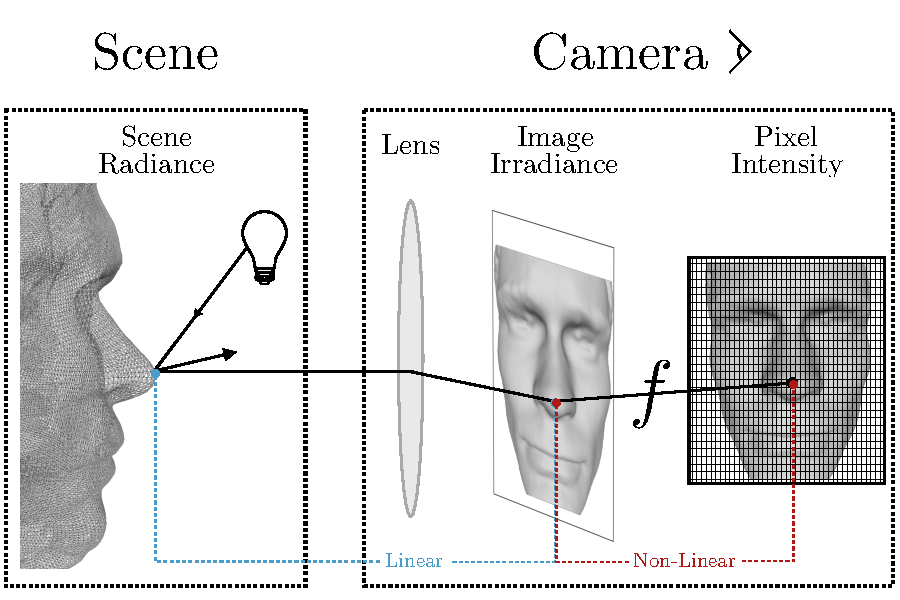
\includegraphics[width=\columnwidth]{background/images/scene_radiance_to_pixel}
	\caption{Illustration of the formation of a pixel intensity in image space
	         from scene radiance. Scene radiance is linearly proportional
	         to image irradiance~\cite{horn1979calculating} and image irradiance
	         is non-linearly mapped to a pixel intensity via the camera
	         response function, $f$.}
\label{fig:bg_sfs_scene_to_intensity}
\end{figure}
%%%%%%%%%%%%%%%%%%%%%%%%%%%%%%%%%%%%%%%%

Even assuming that all of the assumptions outlined above are perfectly
satisfied by an image, SfS is still an under-constrained problem. Given
a single image, $\mathcal{I} \in \R^{w \times h}$ and $d = h \cdot w$, we define
the pixel extraction notation as $\mathcal{I}(x, y)$ which is the scalar
intensity value at the location $(x, y)$ in the image. In the
simple case of an image that depicts a perfectly convex and Lambertian
object with uniform albedo ($\rho_{\smallsub{d}} = 1$), lit by a single
point light of unit flux and known direction that is infinitely far away, the
SfS problem for a single pixel is: $\mathcal{I}(x, y) = {\bb{n}(x, y)}^T \bb{s}$.
Since $\bb{s}$ and $\mathcal{I}(x, y)$ are known, the solution to the problem is a
function of $\bb{n}(x, y)$. An important property of surface normals is that the are
directional vectors that represent local surface orientation. Therefore, they
are parametrised by a unit vector that exists in 3D Cartesian space. However, given the unit norm constraint, surface normals can
also be parametrised as points on the surface of a unit sphere. This is more
evident when normals are converted into spherical coordinates:
%%%%%%%%%%%%%%%%%%%
\begin{equation}\label{eq:bg_sfs_normal_spherical}
    \phi = \arctan{\frac{y}{x}}, \;\;\;\; \theta = \arccos{z}, \;\;\;\; r = 1,
\end{equation}
%%%%%%%%%%%%%%%%%%%
which are clearly a function of two parameters, the azimuth ($\phi$) and
elevation ($\theta$). Similarly, it is common in the SfS literature to
parametrise the surface normals as 2D vectors of the image gradient field:
%%%%%%%%%%%%%%%%%%%
\begin{equation}\label{eq:bg_sfs_normal_pq}
    \bb{n} = \frac{{[p, q, -1]}^T}{\sqrt{p^2 + q^2 + {(-1)}^2}},
\end{equation}
%%%%%%%%%%%%%%%%%%%
where $p = \frac{\partial z}{\partial x}$ and
$q = \frac{\partial z}{\partial y}$ are the parameters of the gradient field
of the surface represented in the image. Therefore, the naive least squares
solution (often termed the \textit{brightness error}) to the SfS problem can be
constructed in matrix form:
%%%%%%%%%%%%%%%%%%%
\begin{equation}\label{eq:bg_sfs_least_squares_lambert}
    \min_{\bb{N}} \lVert \bb{I} - \bb{N} \bb{s} \rVert_F \triangleq
    \min_{\bb{p}, \bb{q}} \lVert \bb{I} - (s_1 \bb{\tilde{p}} + s_2 \bb{\tilde{q}} + s_3 \bb{\tilde{1}}) \rVert_F,
\end{equation}
%%%%%%%%%%%%%%%%%%%
given $d$ is the total number of pixels in the image and
%%%%%%%%%%%%%%%%%%%
\begin{align*}
    \bb{N} &= {[\bb{n}(x_1, y_1), \ldots, \bb{n}(x_w, y_h)]}^T &\in &\R^{d \times 3} \\
	\bb{I} &= {[I(x_1, y_1), \ldots, I(x_w, y_h)]}^T &\in &\R^{d} \\
	\bb{\tilde{p}} &= {\left[\frac{p(x_1, y_1)}{e(x_1, y_1)}, \ldots, \frac{p(x_w, y_h)}{e(x_w, y_h)}\right]}^T &\in &\R^{d} \\
	\bb{\tilde{q}} &= {\left[\frac{q(x_1, y_1)}{e(x_1, y_1)}, \ldots, \frac{q(x_w, y_h)}{e(x_w, y_h)}\right]}^T &\in &\R^{d} \\
 	\bb{\tilde{1}} &= {\left[\frac{1}{e(x_1, y_1)}, \ldots, \frac{1}{e(x_w, y_h)}\right]}^T &\in &\R^{d} \\
	e(x_k, y_k) &= \sqrt{{p(x_k, y_k)}^2 + {q(x_k, y_k)}^2 + 1}. & &
\end{align*}
%%%%%%%%%%%%%%%%%%%
Clearly, this is a function of both $\bb{p}$ and $\bb{q}$ and thus even
the simplest SfS problem is under-constrained. Since
even in the strictest settings SfS is under-constrained, any violations
of the assumptions will only further serve to degrade the recovered shape.

Although surface normals
are a parametrisation of an objects shape, in this thesis we are most
interested in the recovered 3D coordinates. In the case of SfS, this can be
realized as a height map (or depth map) of $z$-coordinates that protrude
from the image plane. Given the $\{p, q\}$ gradient field parametrisation, the
height map may be recovered via integration of the gradient field. However,
due to noise in the gradient field recovery, the gradient field will not be
directly integrable. Therefore, integration of the gradient field into a
surface is itself an area of research. The simplest solution to the
problem is to formulate the integration in terms of the unknown surface,
$\bb{Z}$, and to minimise the least squares error~\cite{horn1990height,simchony1990direct,agrawal2006range}
between the image gradient field and the gradient field of the height map,
$\{\bb{Z}_x, \bb{Z}_y\}$:
%%%%%%%%%%%%%%%%%%%
\begin{equation}\label{eq:bg_sfs_gradient_field_ls}
    \bb{Z} = \int \int {(\bb{Z}_x - \bb{p})}^2 + {(\bb{Z_y} - \bb{q})}^2 \;\; dx dy
\end{equation}
%%%%%%%%%%%%%%%%%%%
which is readily solved via the Poisson equation:
$\nabla^2 \bb{Z} = \operatorname{div}(\bb{p}, \bb{q})$ where
$\operatorname{div}(\bb{p}, \bb{q}) = \frac{\partial p}{\partial x} + \frac{\partial q}{\partial y}$
is the divergence operator. The interested reader should consult the
work of \citet{agrawal2006range}, which provides a unified method for
surface gradient field integration, including the commonly employed Fourier
basis method of \citet{frankot1988method}.

In the following section we review relevant facial SfS algorithms. Unless
explicitly mentioned, the methods below assume that faces exhibit ideal
Lambertian reflectance given by \cref{eg:bg_sfs_lambertian_simple},
which has been shown to be a reasonable approximation
of facial reflectance~\cite{Sirovich:1987te,georghiades2001fromfew,%
Basri:2003ie,turk1991eigenfaces,Hallinan:1994dz,ramamoorthi2002analytic,%
ramamoorthi2001relationship,shashua1997photometric,moses1993face,%
marschner1999image}. For a more
thorough treatment of the generic SfS literature we suggest the surveys
of \citet{zhang1999shape} and \citet{durou2008numerical}.
%%%%%%%%%%%%%%%%%%%%%%%%%%%%%%%%%%%%%%%%%%%%%%%%%%%%%%%%%%%%%%%%%%%%%%%%%%%%%%%%
\subsection{SfS Facial Surface Recovery}
%%%%%%%%%%%%%%%%%%%%%%%%%%%%%%%%%%%%%%%%%%%%%%%%%%%%%%%%%%%%%%%%%%%%%%%%%%%%%%%%
The current state-of-the-art in SfS is the generic method of
\citet{barron2015shape}, called
Shape, Illumination and Reflectance from Shading (SIRFS). The SIRFS method is
described as a generalisation of the modern ``intrinsic image'' algorithm in
which shading is parametrized in terms shape and illumination.
\citet{barron2015shape} seek to recover the most likely explanation, in a
statistical sense, by imposing a set of very general priors around smoothness
and colour composition on the input image. Although this is a state-of-the-art
method, it does not perform well for shape recover of faces.
\citet{li2014intrinsic} extend SIRFS by enforcing facial specific priors. They
use the physically based skin BRDF proposed by \citet{weyrich2006analysis} and
place priors on the skin reflectance parameters using the data
from~\cite{weyrich2006analysis}. They also impose a geometric prior on the face
shape by providing an initial estimate of the 3D face shape
using~\cite{Yang:2011gj}. \citet{li2014intrinsic} show superior results to the
original SIRFS, particular for surface normal recovery.
\citet{atick1996statistical} propose an analysis-by-synthesis method
for minimizing the reconstruction error between a statistical model of facial
surface based on depth images rendered using a Lambertian BRDF and the input
image. Although this is termed as SfS, we classify it as analysis-by-synthesis
and discuss it in further detail in \cref{sec:bg_3dmm}.
\citet{yuan2002sfs} use a neural network in order to constrain the outputs
of a Lambertian SfS algorithm to be in the span of a training set of 3D
depth images.
\citet{fanany2004neural,fanany2002analysis} also propose to use a neural network
for SfM. However, the authors use multiple views of an object and deform
the vertices of a polygonal mesh to be consistent with input from SfS.
\citet{dovgard2004statistical} combine the symmetric SfS method of
\citet{yilmaz2002estimation} with the statistical model of
\citet{atick1996statistical} in order to resolve an ambiguity present in
the symmetric formulation of~\cite{yilmaz2002estimation}.
\citet{smith2010estimating} also use a database of facial surfaces
orthographically projected to form a statistical model of facial shape. They
enforce ``model-based integrability'' by ensuring that normals recovered
by the geometric SfS algorithm of \citet{worthington1999new,Smith:2007eb} lie
in the span of the normals computed from statistical surface model. Furthermore,
\citet{smith2010estimating} show that this framework allows the usage of
more complex BRDFs such as the Phong~\cite{tuong1973illumination} model.
However, although \citet{smith2010estimating} discuss handling non-frontal
illumination, their primary results focus on the case when the illumination
is coincident with the viewing angle.
\citet{biswas2009robust} concentrate on robust albedo estimation, though they
demonstrate the accuracy of their albedo estimation by performing SfS using the
method of \citet{ping1994shape}. In particular, they utilize a mean shape as the
initial shape estimate and thus produce a robust estimate of the albedo using a
Linear Minimum Mean Square Error Estimator (LMMSE). They proceed to normalise
the image using the albedo estimate and then transform the normalised image to
appear lit by the initial illumination direction estimate. Finally, SfS is
performed on the transformed image, which they showed was much more accurate
than performing SfS on the initial input image.
\citet{kemelmacher2011facereconstruction} also utilize a template shape, but
rather than simply initialising a SfS algorithm with this shape, the authors
propose to augment the template geometry with a photometric consistency term
stemming from spherical harmonics. This is similar in spirit to many of the
methods shown in \cref{subsec:bg_capture} where the coarse output of stereo was
augmented with photometric information. 
In \citet{kemelmacher2011facereconstruction} directly optimize over the 3D
surface rather than the normals themselves in order to avoid integration of the
normals as a secondary process. In \citet{kemelmacher2011facereconstruction}, 
the 3D surface is parametrized as a height map and alignment between the input
image and the template mesh is performed via optical flow. This implies that the
method is generally poor at recovering details from posed images as the
alignment between the template and the image must be highly accurate. This work
was also utilized in~\cite{kemelmacher2008mooney} for the recovery of shape
using binary images (dubbed ``Mooney-images'') where the authors show that, with
some consideration, a template mesh may also be deformed to recovery reasonable
facial shape from textureless images.
\citet{roth2015unconstrained} extend the work of~\cite{kemelmacher2011facereconstruction}
by proposing to use a 3D mesh parametrized by vertices rather than as a height
map. 2D facial landmarks are utilized to recover the initial mesh alignment with
the input image and a novel Laplace mesh editing method is used to deform the
template mesh to the photometric normals predicted from the image.
\citet{Suwajanakorn:2014bl} also perturb a template mesh using a photometric
consistency term based on spherical harmonics.
However, \citet{Suwajanakorn:2014bl} deform a person
specific model learnt automatically from Internet images and propose a novel
alignment method they term ``3D-flow''. 3D-flow is an analysis-by-synthesis
method where no statistical constraint is placed on the vertex movements
and thus vertices are free to move in a manner identical to optical flow. In
contrast to other methods described previously, \citet{Suwajanakorn:2014bl}
focus on the recovery of facial shape accurately over sequences.
We note that \citet{nehab2005efficiently} also proposed a general method
for combining coarse templates with normal information.

There are also a number of statistical model based methods that propose the
learning of parametric models of either normals or spherical harmonics.
\citet{smith2006recovering} propose to use a cartographic projection, the
Azimuthal Equidistant Projection (AEP)~\cite{snyder1987map}, to enable
the computation of Principal Component Analysis (PCA) directly on normals. Since
surface normals are vectors it is non-trivial to compute distances between
them. Therefore, the AEP allows PCA to be performed on normals in the tangent
space specified by the projection. Similarly, \citet{smith2008facial} propose
another methodology for computing distances between normals using
Principal Geodesic Analysis (PGA)~\cite{fletcher2004principal}.
Both~\cite{smith2006recovering} and~\cite{smith2008facial} were embedded
in the geometric SfS method of~\cite{worthington1999new} to perform statistical
facial SfS. Similarly, \citet{Ahmad:2011kh} propose to combine the output
from the probabilistic SfS method of \citet{haines2008belief} with the
normals from the statistical model of~\cite{smith2008facial}.
\citet{minsik2009facial} also build a statistical model of surface normals,
but directly on the normals scaled by the albedo, without considering issues
arising from Euclidean distance estimations. PCA is performed on the scaled
normals and then a joint linear model is constructed by weighting the scaled
normals by the lighting coefficients. Several such rotated models are
constructed and at testing time the model with the lowest standard
deviation is chosen to produce the final result. The images are aligned
with an affine alignment using the eye centres and the normals are integrated
using \citet{frankot1988method}.
\cite{minsik2011fast} utilize a tensor decomposition method based on the
2nd order spherical harmonic basis. They compute spherical harmonic
images directly from the surface normals and perform
N-Mode~\cite{vasilescu2003multilinear} on the images of all subjects
to reduce the dimensionality. They then alternately solve for both the
identity mode and the spherical harmonic coefficients to recover the person
specific spherical harmonic images of an input image. Finally, assuming
all images are aligned with an affine alignment, the spherical harmonic
images can be integrated using a method such as~\citet{frankot1988method}.
No further photometric consistency terms are applied.
% TODO: Go through the possible SFS list to see if those citations are
%       relevant or whether they are just relighting papers. At least
%       the tensor splines should be relevant.
%%%%%%%%%%%%%%%%%%%%%%%%%%%%%%%%%%%%%%%%%%%%%%%%%%%%%%%%%%%%%%%%%%%%%%%%%%%%%%%%

%%%%%%%%%%%%%%%%%%%%%%%%%%%%%%%%%%%%%%%%%%%%%%%%%%%%%%%%%%%%%%%%%%%%%%%%%%%%%%%%
\section{Calibrated and Uncalibrated Photometric Stereo}\label{ch:bg_ps}
%%%%%%%%%%%%%%%%%%%%%%%%%%%%%%%%%%%%%%%%%%%%%%%%%%%%%%%%%%%%%%%%%%%%%%%%%%%%%%%%

%%%%%%%%%%%%%%%%%%%%%%%%%%%%%%%%%%%%%%%%%%%%%%%%%%%%%%%%%%%%%%%%%%%%%%%%%%%%%%%%

%%%%%%%%%%%%%%%%%%%%%%%%%%%%%%%%%%%%%%%%%%%%%%%%%%%%%%%%%%%%%%%%%%%%%%%%%%%%%%%%
\section{3D Morphable Models}\label{ch:bg_3dmm}
%%%%%%%%%%%%%%%%%%%%%%%%%%%%%%%%%%%%%%%%%%%%%%%%%%%%%%%%%%%%%%%%%%%%%%%%%%%%%%%%
\cite{atick1996statistical} proposed one of the earliest analysis-by-synthesis
methods for facial shape recovery. They compute PCA on a set of 
Cyberware~\cite{cyberware} scanned heads they are parametrized using
cylindrical coordinates. They then pose shape recovery as the problem
of recovering the PCA coefficients for a given input image by minimizing
the least squares error between the basis rendered orthographically
using a Lambertian BRDF (with assumed known light and uniform albedo) 
and the input image. This work was inspired by the Eigenfaces work of 
\citet{Sirovich:1987te} but utilized 3D data rather than images. To solve
the least squares a linearisation is performed via a Taylor series expansion
and conjugate gradient descent is applied.
%TODO: Check Smith's work and see if there is more stuff
%      for this section. Likely quite a lot of citations 
%      are missing here.
%%%%%%%%%%%%%%%%%%%%%%%%%%%%%%%%%%%%%%%%%%%%%%%%%%%%%%%%%%%%%%%%%%%%%%%%%%%%%%%%

%%%%%%%%%%%%%%%%%%%%%%%%%%%%%%%%%%%%%%%%%%%%%%%%%%%%%%%%%%%%%%%%%%%%%%%%%%%%%%%%
\section{Model-based and Alignment Methods}\label{sec:bg_model_based}
%%%%%%%%%%%%%%%%%%%%%%%%%%%%%%%%%%%%%%%%%%%%%%%%%%%%%%%%%%%%%%%%%%%%%%%%%%%%%%%%
In this section we considered methods that seek to recover 3D by the use
of explicit models of faces. Given some model of the 3D structure of a human
face, it is possible to attempt to find some feature of the input image
that is best matched to some aspect of the model. We separate the literature
into two distinct areas: those that consider reconstruction as a problem of
alignment and those that seek to recover structure from the model assuming
alignment is solved. In contrast to other seemingly similar techniques such as
3D Morphable Models~\cite{volker1999morphable} that use 3D statistical models
of faces the methods considered in this section do not necessarily enforce any
specific structure on the formation of the image.
%%%%%%%%%%%%%%%%%%%%%%%%%%%%%%%%%%%%%%%%%%%%%%%%%%%%%%%%%%%%%%%%%%%%%%%%%%%%%%%%
\subsection{Model-based Methods}\label{subsec:bg_model_based_model}
%%%%%%%%%%%%%%%%%%%%%%%%%%%%%%%%%%%%%%%%%%%%%%%%%%%%%%%%%%%%%%%%%%%%%%%%%%%%%%%%
%TODO: Check Castelan's work
\citet{minsik2013robust} propose a direct mapping from 3D facial shape to an
image of a face under general unknown lighting. The depth and texture pairs from
FRGC~\cite{phillips2005overview} are used to generate a discrete set of
renderings of faces with cast shadows. N-Mode
SVD~\cite{vasilescu2003multilinear} followed by orthogonalisation is applied to
both the rendered textures and the depths in order to perform dimensionality
reduction. This provides a set of transformed images and a subspace is recovered
using a generalised eigenvalue method to further reduce the dimensionality.
Finally, Canonical Correlations Analysis (CCA) is applied between the
dimensionality reduced depth images and a hyperspherical representation of the
image subspace. At test time, the image is transformed using the subspace and
the depth is recovered using the CCA mapping. This process is very fast for
recovery of an input image and handles arbitrary lighting conditions, but
only applies to frontal faces and does not guarantee photometric consistency
of the recovered shape.
\citet{minsik2014realtime} extend the work of \citet{minsik2011fast} with a
novel optimisation procedure that is extremely efficient. Similar
to~\cite{minsik2011fast}, a tensor formulation is proposed. However, the
bilinear model of~\cite{minsik2011fast} is relaxed by enforcing that the
illumination and identity modes can be described as a set of rank-one matrices.
Furthermore, in order to incorporate cast shadows, they render the input meshes
under a variety of illumination conditions including cast shadows and perform
the tensor decomposition on the rendered data rather than the spherical
harmonics, similar to \citet{minsik2013robust}. At test time, the input image
is projected against the bilinear illumination basis and the best rank-one
structure of the lighting and identity coefficients are recovered. The images
are aligned using affine alignment of the eye centres and depth is recovered
from the learnt tensor depth model and the recovered rank-one identity
coefficients.

\cite{Yang:2011gj} require accurate dense 3D shape estimation in order to
perform expression transfer between images. Given a set of known 2D landmarks on
the input image a dense 3D bilinear statistical model is deformed so as to
minimise the re-projection error. Landmarks on the occluding contour are
optimised separately in order to ensure correct 2D-3D correspondences. This
fitting is performed jointly for the two input images in order to attempt to
ensure consistency of identity.
Similarly, \citet{yang2012face} perform 3D expression transfer
but augment the initial 3D shape estimation with a restricted camera model
rather than a weak perspective model.

\citet{Garrido:2013dia} used the 2D facial landmarking method of
\citet{saragih2011deformable} to track a set of sparse feature points across
a sequence. Key frames are detected as frames where the 2D landmarking was
deemed accurate, according to the difference between the frame and a neutral
frame. Optical flow is used to correct the 2D landmarks and pose and blend shape
optimisation are iterated to perform 3D tracking. Finally, the tracked
blend shape is deformed by the optical flow estimates and a Shape-from-Shading
refinement method~\cite{valgaerts2012lightweight} is used to include finer
surface detail such as wrinkles.

\citet{ferrari2015dictionary} used the method of
\citet{xiong2013supervised} to provide sparse 2D landmarks and perform
an alternating ridge regression to solve for pose and the parameters of a sparse
dictionary of dense 3D faces.
%TODO: Shape-from-silhoette and shape-from-contours both fall in this section
%      due to the fact that all the methods I can find use models!
%%%%%%%%%%%%%%%%%%%%%%%%%%%%%%%%%%%%%%%%%%%%%%%%%%%%%%%%%%%%%%%%%%%%%%%%%%%%%%%%
\subsection{Alignment Methods}\label{subsec:bg_model_based_alignment}
%%%%%%%%%%%%%%%%%%%%%%%%%%%%%%%%%%%%%%%%%%%%%%%%%%%%%%%%%%%%%%%%%%%%%%%%%%%%%%%%
Alignment based 3D recovery methods attempt to recover the best possible
reconstruction of an input model for an input image. Unlike purely model
driven methods, alignment algorithms assume that the initialisation will not be
perfect and thus attempt to deform the model in some manner in order to best
replicate some feature of the input image. Unlike 3DMMs, alignment methods
do not necessarily try to synthesize the image, but instead focus on learning
relationships between some feature of the image and the model.

\cite{terzopoulos1993analysis} build a physics based synthetic tissue model
for a sparse generic 3D model coupled with a set of anatomically motivated
muscle activators. Contours are extracted from input images and the physically
based model is used to deform the generic mesh. Similarly,
\citet{essa1997coding} use a low vertex generic face mesh and augment it with
an anatomically based muscles model. This model uses the Facial Action Coding
System (FACS)~\cite{ekman1977facial} to parametrise face motion. Landmarks
are used to initialise the face model onto a frontal face and then optical
flow is performed. The displacements recovered by optical flow from a
neutral pose are then fed into an optimisation that deforms the mesh according
to the physically based muscle model.
\citet{jebara1997parametrized} track the 3D motion of a face using a generic
dense 3D face mesh and a modified rigid Structure-from-Motion algorithm
to recover the head pose. Symmetric frontalisation is performed on the face
within the image and an Extended Kalman Filter (EKF) is used to perform motion
updates that are consistent for the 3D model. The EKF is filtered by an
eigenspace of frontalised 3D faces to constraint the tracking to plausible face
shapes.
\citet{basu1996motion} regularise optical flow with an ellipsoidal mesh
to approximate a facial shape, which they show to be superior to planar
tracking.
\citet{lacascia1998head,la2000fast} do not concentrate on 3D reconstruction but
perform 3D head tracking by approximating the head shape as a cylinder and
performing alignment in the texture mapped space. In \citet{la2000fast} this
is extended with a statistical model of illumination variance built from
many aligned images of various individuals under differing illumination.
\cite{schoedl1998head} used a more realistic textured model than
\citet{lacascia1998head} and employ a low vertex count 3D generic face model. A
single frontal texture is extracted and used in an ``analysis-by-synthesis''
manner to minimise the difference between the input image and the rendered
model.
\citet{decarlo2000optical} employ a sparse generic model that is parametrically
deformed by a set of static shape parameters and motion deformation
parameters. The model is initialised by hand on a neutral frontal image and
optical flow is then employed for tracking. The parameters of the
3D deformable motion model are hard constrained by the result of the flow.
To combat tracking drift, image edge features are introduced as another
constraint.
\cite{decarlo2002adjusting} extends the work of \citet{decarlo2000optical} with
an extra regularisation based on minimising the residual error from the
framework of \citet{decarlo2000optical}. Minimising these residuals with respect
to a linearisation of the model parameters results in a more robust recovery of
the facial shape and thus reduces the optical flow residual in a manner
consistent with facial deformations.
\citet{goldenstein2004facial} focus on the estimation of the update for
the deformable model by using multiple image features (optical flow,
edges, feature points) and assume their independence. The independence
of these features enables the use of a multivariate Gaussian approximation
to estimate displacements using a Kalman filter.
\citet{pighin2002modeling} manually specify a set of landmarks and deform
a single dense generic template head to multiple poses images of a subject.
Rigid Structure-from-Motion is used to estimate the head pose, initialised
by the rough estimate of the known pose of the face \eg~side-view, frontal \etc.
All the vertices in the generic mesh are then deformed by landmarks
using a radial basis function including an additional 100 correspondences
that are hand specified and a view-independent texture is created from the input
images. This person specific model is then fit to an input
sequence by using a non-linear least squares algorithm similar to the Active
Appearance Model (AAM) but with a 3D model. The ``analysis-by-synthesis''
objective involves rendering the input mesh but no lighting conditions are
modelled.

\citet{lie2006alignment} propose to model a 3D face as a set of sparse patches
rendering from the 3D model over various poses. An expectation maximisation
method is proposed to predict the parameters of a sparse 3D statistical face
model (deformation) and pose parameters from a given 2D observation. Pose
and deformation are solved for alternately.
\cite{Matthews:2007gb} provide a detailed analysis on the advantages
of imposing 3D priors for Active Appearance Model alignment. They propose to
build the 2D statistical model from samples of a projected 3D model and then
to constrain the 2D fitting by the 3D model. The 3D model is sparse and learnt
via Structure-from-Motion on the training set. \citet{Ramnath:2008jp} extend
\cite{Matthews:2007gb} in order to perform alignment on multiple posed
images of an individual. By leveraging the additional information from
multiple images they show improved fitting performance across all views.
\cite{Martins:2013hp} also propose a 3D AAM, but employ a fully perspective
camera model and show how to optimise via a 3D perspective projection
using a forward additive alignment algorithm. Therefore, no intermediate
2D model is required. Similarly, \citet{saragih2011real} extend their 2D
face alignment work~\cite{saragih2011deformable} on Constrained Local Models
(CLMs)~\cite{cristinacce2006feature} to fit a 3D CLM.\@ These sparsely
tracked points were primarily demonstrated for avatar animation.
\cite{Liao:2010fy} use both raw pixel intensities as well as
SIFT~\cite{lowe2004distinctive} as input to an inverse compositional alignment
algorithm~\cite{baker2004lucas} evaluated for face tracking. The SIFT features
are required to be distant from one another and matched features must be close
between frames.
\citet{Wang:2011kr} propose a one-shot optimization approach to simultaneously
estimate the sparse 3D landmarks, the corresponding 2D projections and their
visibility states without requiring explicit estimation of the camera
parameters. A higher order Markov Random Field (MRF) is used to encode the
outputs and optimised via a dual-decomposition optimisation
framework~\cite{komodakis2007mrf}.

\printauthor{Cao:2013cd} proposed a series of works for efficient blend shape
tracking from a monocular sequence. Using their collected database,
FaceWarehouse~\cite{Cao:2014gy}, \citet{Cao:2013cd} first proposed a person
specific method for 3D face tracking. A person specific regressor was learnt
from a set of acted expressions in order to map 2D facial images to 3D blend
shape parameters. This initial recording specific training was important in
order to learn the cameras intrinsic parameters. In \citet{Cao:2014bi}, the
authors relax the requirement for a person specific calibration process and
propose to learnt the camera intrinsic and subject identity parameters in an
online manner. Using the same 3D regression scheme as in
\citet{Cao:2013cd}, the camera and identity parameters are updated online when
a new representative frame is detected. These frames are detected via distance
from a PCA subspace that is maintained online. Thus the identity and camera
intrinsics are shown to converge over the coarse of an input sequence. Both
\citet{Cao:2013cd} and \citet{Cao:2014bi} use the two-stage cascaded regression
scheme proposed by \citet{cao2014face} to learnt the regression between the
input image and the model parameters. More recently, the work from
\citet{Cao:2014bi} has augmented with a real-time high frequency feature
displacement method by \citet{Cao:2015gy}. Given the coarse geometry recovered
by \citet{Cao:2014bi}, the authors of~\cite{Cao:2015gy} augment the geometry
to include both wrinkles and simple mesoscopic features captured by a narrow
band Difference of Gaussians (DoG) filter~\cite{Beeler:2010dg}. They also
further refine the geometry via GPU Lucas-Kanade~\cite{lucas1981iterative}
optical flow algorithm between each frame. \citet{Chai:2015dq} also
utilised \citet{Cao:2014bi} in order to recover 3D geometry for an input image
to supplement their novel hair synthesis method.

In recent years, cascaded regression methods have become popular for approaching
2D image alignment~\cite{xiong2013supervised,cao2014face,ren2014face,kazemi2014one}.
Given the increased availability to varied 3D face databases, recent works have
directly extended these cascaded alignment methods in order to train 3D cascaded
regression algorithms. \citet{tulyakov2015regressing} train on sparse 3D
landmarks from the BU4D-FE~\cite{yin2008high} and directly extend the method
\citet{kazemi2014one} into 3D. The training set consists of rendered examples
from BU4D-FE.\@ They do not explicitly handle the camera projection and instead
estimate it from the mean shape.
\citet{Jeni:2015ft} propose a semi-dense 2D landmark alignment method that is
learnt from the 3D meshes provided by the BU4D-FE~\cite{yin2008high} and BP4D-
Spontaneous~\cite{Zhang:2014id} databases. At alignment time, only 2D landmarks
are considered and a secondary alternating pose and parameter recovery method is
used to recover 3D shape~\cite{lie2006alignment}. The training set consists of
rendered examples from the database.
\citet{Jourabloo:2015dw} also recover sparse landmarks but they consider a two-
stage regression to regress both the parameters of the 3D shape model and the
camera projection matrix separately. The 3D shape model is learnt from 3D facial
scans and the AFLW~\cite{kostinger2011annotated} database is used to learn the
regressors.
\citet{zhu2015discriminative} use the FRGC~\cite{phillips2005overview} database
to learn both the 3D statistical shape model and the 2D-3D regression. Camera
and shape model parameters are regressed jointly and the method is initialised
by the output of the SDM method~\cite{xiong2013supervised}.
\citet{Huber:2015bs} use a statistical model learnt from the
SURREY~\cite{Huber:F5Dca9zy} database and also jointly regress the camera and
dense shape model parameters. However, no examples of the 3D recovery are given.
All of the aforementioned methods learn to regress from local features extracted
around projections of the 3D model into the image plane. In contrast,
\citet{Zhu:2015ur} use a Convolutional Neural Network (CNN) to learnt a holistic
representation based on all of the input pixels within the original detected
facial bounding box. They also propose to use a set of mesh features from the
current Z-buffered projection of the dense shape estimate and concatenate these
features into a multi-channel image with the texture features. They propose a
novel cost function for jointly optimising the camera and shape model parameters
in a weighted manner. The 3D shape model is bilinear in expression and identity
and is thus built from the FaceWarehouse~\cite{Cao:2014gy} and
Basel~\cite{paysan20093d} databases respectively.
%TODO: Include puppeteering/expression synthesis as its probably most relevant
%      either here or in model-based.
%%%%%%%%%%%%%%%%%%%%%%%%%%%%%%%%%%%%%%%%%%%%%%%%%%%%%%%%%%%%%%%%%%%%%%%%%%%%%%%%

%%%%%%%%%%%%%%%%%%%%%%%%%%%%%%%%%%%%%%%%%%%%%%%%%%%%%%%%%%%%%%%%%%%%%%%%%%%%%%%%
\section{Structure-from-Motion}\label{ch:bg_sfm}
%%%%%%%%%%%%%%%%%%%%%%%%%%%%%%%%%%%%%%%%%%%%%%%%%%%%%%%%%%%%%%%%%%%%%%%%%%%%%%%%
%TODO: This will be quite hard to nail down outside of
%      Tassos' work. May need his advise.
%TODO: Check references 75-86 of 
%      A SURVEY ON 3D MODELING OF HUMAN FACES FOR FACE RECOGNITION
%%%%%%%%%%%%%%%%%%%%%%%%%%%%%%%%%%%%%%%%%%%%%%%%%%%%%%%%%%%%%%%%%%%%%%%%%%%%%%%%

%%%%%%%%%%%%%%%%%%%%%%%%%%%%%%%%%%%%%%%%%%%%%%%%%%%%%%%%%%%%%%%%%%%%%%%%%%%%%%%%
\stopcontents[chapters]
%%%%%%%%%%%%%%%%%%%%%%%%%%%%%%%%%%%%%%%%%%%%%%%%%%%%%%%%%%%%%%%%%%%%%%%%%%%%%%%%